\documentclass[aps,pra,10pt,twocolumn,superscriptaddress,nofootinbib,floatfix]{revtex4-2}
\usepackage[T1]{fontenc}
\usepackage{lmodern}
\usepackage{amsmath,amssymb,amsthm,bm,graphicx,xcolor}
\usepackage[colorlinks=true,linkcolor=blue!45!black,citecolor=blue!45!black,urlcolor=blue!45!black]{hyperref}

\newtheorem{theorem}{Theorem}
\newtheorem{lemma}{Lemma}
\newtheorem{proposition}{Proposition}
\newtheorem{corollary}{Corollary}
\theoremstyle{definition}
\newtheorem{definition}{Definition}
\theoremstyle{remark}
\newtheorem{remark}{Remark}

%% generated by make_numbers.py from out/results.json; do not edit
\newcommand{\nRoutes}{63}
\newcommand{\nChecked}{38}
\newcommand{\nFailed}{0}
\newcommand{\nExact}{21}
\newcommand{\nLogic}{3}
\newcommand{\nNumeric}{13}
\newcommand{\nImportChecked}{1}
\newcommand{\nImported}{6}
\newcommand{\nDefinitions}{4}
\newcommand{\nWritten}{15}
\newcommand{\nNodes}{35}
\newcommand{\nReleased}{17}
\newcommand{\nNew}{18}
\newcommand{\nS}{10}
\newcommand{\nM}{13}
\newcommand{\nO}{12}
\newcommand{\nControls}{16}
\newcommand{\nControlsRejected}{16}
\newcommand{\nClaims}{11}
\newcommand{\runSeconds}{38}
\newcommand{\verPython}{3.13.18}
\newcommand{\verSympy}{1.14.0}
\newcommand{\verNumpy}{2.5.3}
\newcommand{\verScipy}{1.18.1}
\newcommand{\verCvxpy}{1.9.3}
\newcommand{\verZthree}{5.4.1}
\newcommand{\mtop}{172.60}
\newcommand{\mtopErr}{0.27}
\newcommand{\mW}{80.3625}
\newcommand{\mWErr}{0.0077}
\newcommand{\kappab}{0.395}
\newcommand{\kappanu}{0.336}
\newcommand{\kappanuErr}{0.002}
\newcommand{\kappabBSU}{0.406}
\newcommand{\kappanuBSU}{0.318}
\newcommand{\xistar}{4.634}
\newcommand{\mtstar}{173.0}
\newcommand{\mtstarFine}{172.99}
\newcommand{\mtstarPull}{1.4}
\newcommand{\twomW}{160.7}
\newcommand{\cnorm}{1.108}
\newcommand{\cnormAvg}{1.109}
\newcommand{\cnormErr}{0.009}
\newcommand{\cosc}{0.517}
\newcommand{\coscLo}{0.501}
\newcommand{\coscHi}{0.535}
\newcommand{\fracEvents}{46.5}
\newcommand{\alphaprod}{0.568}
\newcommand{\alphapsi}{0.4748}
\newcommand{\dphi}{0.7521}
\newcommand{\alpham}{0.7519}
\newcommand{\alphap}{-0.7559}
\newcommand{\wzeroLambda}{0.151}
\newcommand{\zATLAS}{10.2}
\newcommand{\zCMS}{5.1}
\newcommand{\lpRlo}{1.0001}
\newcommand{\lpRhi}{1.0079}
\newcommand{\lpRtwolo}{0.9879}
\newcommand{\lpRtwohi}{1.0086}
\newcommand{\lpRdirs}{12}
\newcommand{\lpRtwodirs}{9}
\newcommand{\lpRK}{220}
\newcommand{\lpRnq}{900}
\newcommand{\lpRtwoK}{264}
\newcommand{\lpRtwonq}{700}
\newcommand{\refA}{1.0069}
\newcommand{\refB}{1.0019}
\newcommand{\refC}{1.0100}
\newcommand{\refD}{1.0022}
\newcommand{\refE}{0.9879}
\newcommand{\refF}{1.0001}
\newcommand{\refAnq}{900}
\newcommand{\refBnq}{3600}
\newcommand{\refCnq}{700}
\newcommand{\refDnq}{2800}
\newcommand{\bracketN}{250}
\newcommand{\bracketWidth}{0.023}
\newcommand{\sdpDev}{8.4\times 10^{-9}}
\newcommand{\gjDev}{3.8\times 10^{-7}}
\newcommand{\etaStarMin}{0.013}
\newcommand{\taurho}{0.449}
\newcommand{\Ae}{0.1515}
\newcommand{\AeErr}{0.0019}
\newcommand{\wzeroSigma}{0.605}
\newcommand{\wzeroSigmaErr}{0.005}
\newcommand{\zSigma}{1.1}
\newcommand{\zLambdaKernel}{39}
\newcommand{\alphaSigma}{-0.508}
\newcommand{\alphaSigmaErr}{0.007}
\newcommand{\xtau}{0.232}
\newcommand{\alphatau}{0.037}
\newcommand{\cnormSigma}{1.99}
\newcommand{\cnormSigmaErr}{0.11}
\newcommand{\zcnorm}{12}
\newcommand{\kbsq}{0.156}
\newcommand{\Cneed}{2.53}
\newcommand{\alphapsiErr}{0.0038}
\newcommand{\dphiErr}{0.0078}
\newcommand{\alphamErr}{0.0043}
\newcommand{\alphapErr}{0.0047}
\newcommand{\DATLAS}{-0.537}
\newcommand{\DATLASbound}{-0.322}
\newcommand{\DCMS}{-0.480}
\newcommand{\trcCMS}{1.44}


\newcommand{\Tr}{\operatorname{Tr}}
\newcommand{\tr}{\operatorname{tr}}
\newcommand{\conv}{\operatorname{conv}}
\newcommand{\bq}{\bm{q}}
\newcommand{\bn}{\bm{n}}
\newcommand{\bp}{\bm{p}}
\newcommand{\bv}{\bm{v}}
\newcommand{\bt}{\bm{t}}
\newcommand{\bb}{\bm{b}}
\newcommand{\ba}{\bm{a}}
\newcommand{\bx}{\bm{x}}
\newcommand{\bz}{\bm{z}}
\newcommand{\bu}{\bm{u}}
\newcommand{\bP}{\bm{P}}
\newcommand{\bS}{\bm{S}}
\newcommand{\bJ}{\bm{J}}
\newcommand{\bsig}{\bm{\sigma}}
\newcommand{\cK}{\mathcal{K}}
\newcommand{\cR}{\mathcal{R}}
\newcommand{\cQ}{\mathcal{Q}}
\newcommand{\cE}{\mathcal{E}}
\newcommand{\cF}{\mathcal{F}}
\newcommand{\rhoraw}{\rho_{\mathrm{raw}}}
\newcommand{\Rraw}{R}
\newcommand{\T}{\mathsf{T}}
\newcommand{\node}[1]{\texttt{#1}}
\newcommand{\inlinecaption}[2]{\refstepcounter{table}\label{#1}\begin{center}\small TABLE~\thetable. #2\end{center}\vspace{-1ex}}

\begin{document}

\title{Particle decays as fixed measurements: exact noncontextuality thresholds for decay-angle correlations}

\author{Tahmeed Hossain}
\affiliation{Department of Theoretical Physics, University of Dhaka, Dhaka, Bangladesh}

\date{17 November 2026. \textbf{Generated work} produced with Claude (Anthropic); unpublished, not peer reviewed.}

\begin{abstract}
A particle decay records the spin of its parent through one fixed rotation-covariant measurement.
Data taken with one such measurement per particle cannot violate a Bell or a steering inequality, because the recorded directions themselves serve as local hidden variables.
We ask instead whether the data admit a generalized-noncontextual ontological model, and answer exactly.
For a spin-$1/2$ particle with polarisation $P$ and spin analysing power $\kappa$ a model exists if and only if $P|\kappa|\le 1/3$.
For two spin-$1/2$ particles it exists if and only if the operator $\rhoraw$ assembled from the raw angular coefficients, not divided by the analysing powers, is positive with positive partial transpose; for unpolarised pairs this reads $\|c\|_1\le 1$, and it implies $|D|\le 1/3$ for the opening-angle coefficient.
For spin $1$ the helicity weights of noncontextual polarimeters form, in the plane of vector and tensor analysing ratios, the convex hull of an ellipse and a point; for a spin-singlet pair of spin-$1$ particles the admissible products of ratios form a second region bounded by parabolic arcs, and two ideal $W\to\ell\nu$ decays give contextual data if and only if the singlet visibility exceeds $5/8$.
For spin $j$ the largest vector analysing power of a noncontextual polarimeter is the largest node $\xi_{2j}$ of a Gauss--Legendre (integer $j$) or Gauss--Radau (half-integer $j$) quadrature rule, and for two particles of any spins and in any state noncontextual data obey $\|\langle\bq_A\bq_B^{\T}\rangle\|_1\le\xi_{2j_A}\xi_{2j_B}$ for the matrix of first moments of the two recorded directions.
Consequences: the direction-only electron asymmetry of muon decay lies exactly on the threshold; the $b$-quark direction is a nonclassical top-quark polarimeter if and only if $m_t>2m_W$ at leading order; the measured top-pair coefficient $D$ excludes noncontextual models at the significance quoted for entanglement, with no input on the analysing power; with the BESIII fit parameters the $p\bar p$ angular data of $J/\psi\to\Lambda\bar\Lambda$ are contextual for $|\cos\theta|<\cosc$, although the pair is entangled at all production angles.
The results are recorded as routes of a three-layer concept graph (states, models, observables): \nChecked\ of \nRoutes\ routes carry executable certificates, \nWritten\ are proofs written in this paper, and \nControlsRejected\ of \nControls\ planted errors are rejected.
\end{abstract}

\maketitle

\section{Introduction}

Spin correlations of unstable particles are measured through the angular distributions of their decay products. On this basis entanglement has been reported for top-quark pairs at the LHC \cite{atlas2024,cms2024,cms2024ljets}, following the proposal of Ref.~\cite{afik2021}, and a wider programme has formed around top quarks, $\tau$ leptons, hyperons and massive gauge bosons \cite{barr2024,ashby2023,tornqvist1981,besiii2025}.

It has been known since the first proposals that such data cannot test local realism \cite{abel1992}. Each particle is measured by its own decay, that is, with a single setting; all recorded quantities commute; and the recorded momenta themselves constitute a local hidden-variable model. The point has recently been restated and sharpened \cite{abel2025,bechtle2025,low2025}, and what can still be inferred has been discussed in Refs.~\cite{li2024,fabbrichesi2025bell}. What the measured coefficients do establish is entanglement of the reconstructed spin state, given the quantum description of the decay and in particular the value of its spin analysing power.

This paper addresses a question that is well posed for one fixed measurement. A decay is a rotation-covariant positive-operator-valued measure (POVM) on the spin of the parent, with a continuum of outcomes. Many functions of the outcome define the same effect: the angular distribution of a spin-$j$ parent contains spherical harmonics of degree at most $2j$, so every function of the recorded direction that is orthogonal to these integrates to the zero operator. Such operational equivalences are what a generalized-noncontextual ontological model \cite{spekkens2005} must respect: equivalent preparations are represented by the same distribution over ontic states, equivalent effects by the same response function. The existence of such a model is a notion of classical explainability with several equivalent forms: simplex embeddability of the accessible fragment \cite{schmid2021,gitton2022,selby2023frag}, which is decidable by a linear programme \cite{selby2024lp}, and nonnegativity of some quasiprobability representation \cite{spekkens2008}. It can fail for a single measurement \cite{selby2023incomp}, and for a bipartite state with all local measurements available it fails exactly when the state is entangled \cite{plavala2024}. The recorded-outcome model of Refs.~\cite{abel1992,abel2025} is not of this kind: it assigns different response functions to equivalent effects (Sec.~\ref{sec:models}).

We determine exactly when decay data admit a noncontextual model.

(i) \emph{Spin $1/2$, one particle.} With polarisation $P$ and analysing power $\kappa$ a model exists if and only if $P|\kappa|\le 1/3$ (Theorem~\ref{thm:half}).

(ii) \emph{Two spin-$1/2$ particles.} Write the joint distribution of the two recorded directions as $(4\pi)^2p=1+\ba\!\cdot\!\bq_A+\bb\!\cdot\!\bq_B+\bq_A^{\T}c\,\bq_B$. A model exists if and only if the operator $\rhoraw=\tfrac14(\openone+\ba\!\cdot\!\bsig\otimes\openone+\openone\otimes\bb\!\cdot\!\bsig+\sum_{ik}c_{ik}\sigma_i\otimes\sigma_k)$ is positive semidefinite and has a positive partial transpose (Theorem~\ref{thm:pair}). The test uses the raw coefficients; the entanglement test uses the coefficients divided by $\kappa_A\kappa_B$. Contextual data imply an entangled state, and the converse holds for all states only if $|\kappa_A\kappa_B|=1$.

(iii) \emph{Spin $1$.} A decay is specified by helicity weights $(w_+,w_0,w_-)$, equivalently by the vector and tensor ratios $\eta_1=w_+-w_-$ and $\eta_2=1-3w_0$. On all spin-$1$ states a model exists if and only if $(\eta_1,\eta_2)$ lies in the convex hull $\cR$ of the ellipse $3\eta_1^2+25(\eta_2-\tfrac15)^2\le1$ and the point $(0,-\tfrac45)$ (Theorem~\ref{thm:one}). For a spin-singlet pair with one decay on each side the products of the ratios must lie in a second region $\cR_2$ (Theorem~\ref{thm:onepair}).

(iv) \emph{Spin $j$.} The largest vector analysing power of a noncontextual polarimeter is the largest node of the Gauss--Legendre rule with $j+1$ nodes (integer $j$) or of the Gauss--Radau rule with $j+\tfrac32$ nodes (half-integer $j$): $\xi_{2j}=1/3$, $1/\sqrt3$, $(1+\sqrt6)/5$, $\sqrt{3/5}$ for $j=\tfrac12,1,\tfrac32,2$ (Theorem~\ref{thm:spinj}). For two particles of arbitrary spins a noncontextual model is a local model whose response functions are nonnegative polynomials of degree $2j$ in the recorded direction (Proposition~\ref{prop:pairpoly}), which implies $\|\langle\bq_A\bq_B^{\T}\rangle\|_1\le\xi_{2j_A}\xi_{2j_B}$ for the matrix of first moments, whatever the state and the decays.

(v) \emph{Data.} Section~\ref{sec:apps} applies these statements to the decays of muons, $\tau$ leptons and top quarks, to the top-pair coefficient $D$ measured by ATLAS and CMS, to the BESIII parameters of $J/\psi\to\Lambda\bar\Lambda$, and to decays of vector bosons and vector mesons.

\emph{Relation to earlier work.} Fucci \emph{et al.}~\cite{fucci2026} construct Bell tests for decay processes in which independently sampled analysis axes play the role of settings and detector regions give binary or null outcomes; a violation requires postselection, and they show that a local model exploiting it must be measurement contextual, with an inequality violated when the effective analysing powers are large enough. Here no auxiliary settings and no postselection are introduced: the object is the fragment formed by the recorded directions themselves, and the conditions are necessary and sufficient. Fabbrichesi \emph{et al.}~\cite{fabbrichesi2025pra,fabbrichesi2025prd} evaluate Kochen--Specker-type inequalities on spin density matrices reconstructed from collider data; the measurements entering those inequalities are projective spin measurements evaluated on the reconstructed state, not the decay. Li, Shen and Yang~\cite{li2024} exclude a class of hidden-variable models with classical spins and known analysing powers. The equivalence of entanglement and contextuality for all local measurements \cite{plavala2024} becomes a strict implication here because a decay supplies one measurement. For a single qubit our threshold is the entanglement-breaking threshold of the depolarising map \cite{horodeckiEB2003,ruskai2003}; noise thresholds for preparation noncontextuality alone are weaker \cite{marvian2020}, and the classification of individual processes by generalized noncontextuality is developed in Ref.~\cite{zhang2025prx}. Related notions of operational contextuality, including contextuality revealed by a single measurement, are studied in Refs.~\cite{jokinen2024,jokinen2026}.

\emph{The graph.} The question arose from two released concept graphs, each with a state, a model and an observable layer. Their convention is that a relation known in the literature is an edge; the charged-current vertex of the particle-physics graph \cite{genhep} and the generalized-contextuality node of the Nonclassicality Network \cite{gengpt} were not connected. The statements of this paper are the routes that connect them, through new nodes for the decay polarimeter, the steered ensembles and the tests. Each route has a grade (exact, logic, numeric, import, definition, or written proof) and, where possible, an executable certificate; Sec.~\ref{sec:graph} and Appendix~\ref{app:catalogue} give the encoding and the results of the checks.

\section{Decays as measurements, and their classical models}
\label{sec:setting}

\subsection{The decay polarimeter}
\label{sec:polarimeter}

Let $\rho$ be the spin density operator of a particle of spin $j$ in its rest frame, on $\mathbb{C}^d$ with $d=2j+1$. Fix a decay channel and a final-state momentum whose direction $\bq$ (a unit vector in the rest frame of the parent) is recorded. By the Born rule the probability density of $\bq$ is
\begin{equation}
p(\bq)=\Tr[\rho\,E(\bq)],\qquad E(\bq)\ge0,\qquad \int\! d\bq\,E(\bq)=\openone ,
\label{eq:born}
\end{equation}
with $d\bq$ the area element of the unit sphere. If the decay interaction is rotation invariant and nothing else is recorded, $E(R\bq)=U_RE(\bq)U_R^\dagger$ for every rotation $R$, so that
\begin{equation}
E_w(\bq)=\frac{d}{4\pi}\,U_{\bq}D_wU_{\bq}^\dagger,\qquad D_w=\sum_{m=-j}^{j}w_m\,|j,m\rangle\langle j,m| ,
\label{eq:povm}
\end{equation}
where $U_{\bq}$ is any rotation taking the $z$ axis to $\bq$, $w_m\ge0$ and $\sum_mw_m=1$. The weight $w_m$ is the probability that the recorded direction carries projection $m$ of the parent spin; for a two-body decay with helicity amplitudes $A_{\lambda_1\lambda_2}$ \cite{jacob1959}, $w_m=\sum_{\lambda_1-\lambda_2=m}|A_{\lambda_1\lambda_2}|^2/\sum|A_{\lambda_1\lambda_2}|^2$ with $\bq$ the direction of particle~1. We call $w$ the \emph{kernel} and the POVM \eqref{eq:povm} the \emph{decay polarimeter}. If rotation-invariant variables $x$ are recorded in addition (energies, invariant masses), there is one kernel $w(x)$ for each value, and the direction-only kernel is their average.

Decompose operators on $\mathbb{C}^d$ into irreducible tensor components of rank $l=0,\dots,2j$ and let $\Pi_l$ be the projector onto rank $l$. The coherent projector $|j,j\rangle\langle j,j|$ has a nonzero diagonal component of every rank. The \emph{multipole ratios} of a kernel are the numbers $\eta_l(w)$ defined by $\Pi_l[D_w]=\eta_l(w)\,\Pi_l[\,|j,j\rangle\langle j,j|\,]$; $\eta_0=1$. With $\Lambda_\eta=\sum_l\eta_l\Pi_l$ and the coherent states $|\bq\rangle=U_{\bq}|j,j\rangle$,
\begin{equation}
\begin{aligned}
E_w(\bq)&=\Lambda_\eta\Big[\frac{d}{4\pi}|\bq\rangle\langle\bq|\Big],\\
\Tr[XE_w(\bq)]&=\frac{d}{4\pi}\,\langle\bq|\Lambda_\eta X|\bq\rangle .
\end{aligned}
\label{eq:lambda}
\end{equation}
The function $Q_X(\bq)=\langle\bq|X|\bq\rangle$ is the Husimi function of $X$ \cite{radcliffe1971}; it is a polynomial of degree at most $2j$ in the components of $\bq$. The first ratio is the \emph{vector analysing power}
\begin{equation}
\kappa_1\equiv\eta_1=\frac1j\sum_mm\,w_m,\qquad \int\! d\bq\;\bq\,E_w(\bq)=\frac{\kappa_1}{j+1}\,\bJ ,
\label{eq:firstmoment}
\end{equation}
so that $p(\bq)=\frac{1}{4\pi}\big[1+\frac{3j}{j+1}\kappa_1\,\bP\!\cdot\!\bq+\dots\big]$ with $\bP=\langle\bJ\rangle/j$ and the dots standing for harmonics of degree $2,\dots,2j$.

\emph{Spin $1/2$.} $D_w=\tfrac12(\openone+\kappa\sigma_z)$ with $\kappa=w_+-w_-$, and
\begin{equation}
E(\bq)=\frac{1}{4\pi}\,(\openone+\kappa\,\bq\!\cdot\!\bsig),\qquad p(\bq)=\frac{1}{4\pi}\,(1+\kappa\,\bP\!\cdot\!\bq).
\label{eq:half}
\end{equation}
This is the standard definition of the spin analysing power (the decay parameter $\alpha$ of hyperons \cite{leeyang1957}).

\emph{Spin $1$.} With $\eta_1=w_+-w_-$ and $\eta_2=1-3w_0$,
\begin{equation}
U_{\bq}D_wU_{\bq}^\dagger=\frac13+\frac{\eta_1}{2}\,\bq\!\cdot\!\bS+\frac{\eta_2}{6}\big[3(\bq\!\cdot\!\bS)^2-2\big].
\label{eq:spin1kernel}
\end{equation}
A unit-trace Hermitian operator $X$ is specified by $\bp=\Tr[X\bS]$ and the symmetric traceless matrix $A_{ik}=\Tr[X(\tfrac12\{S_i,S_k\}-\tfrac23\delta_{ik})]$, and
\begin{equation}
\Tr[X\,U_{\bq}D_wU_{\bq}^\dagger]=\frac13+\frac{\eta_1}{2}\,\bp\!\cdot\!\bq+\frac{\eta_2}{2}\,\bq^{\T}A\,\bq .
\label{eq:symbol}
\end{equation}

\subsection{Kernels from the charged-current vertex}
\label{sec:va}

Consider the amplitude
\begin{equation}
\mathcal{M}=[\bar u(p_2)\gamma^\mu P_Lu(p_1,s)]\,[\bar u(p_3)\gamma_\mu P_Lv(p_4)],
\label{eq:amp}
\end{equation}
with $P_L=\tfrac12(1-\gamma^5)$, massless fermions 2, 3, 4, and a parent of mass $m$ with spin four-vector $s$. Summed over the spins of the decay products,
\begin{equation}
\sum|\mathcal{M}|^2=8\,[(p_1-ms)\!\cdot\!p_4]\,(p_2\!\cdot\!p_3).
\label{eq:trace}
\end{equation}
In the rest frame of the parent $(p_1-ms)\!\cdot\!p_4=mE_4\,(1+\hat{\bm s}\!\cdot\!\bq_4)$. Hence, at every value of the other kinematic variables and for any propagator depending on invariants only, the direction of the antifermion of the second current is recorded by the rank-one effect $(\openone+\bq\!\cdot\!\bsig)/4\pi$: $\kappa=1$. This is the charged lepton or the down-type quark of a top-quark decay. For the fermion of the second current (the electron of $\mu^-\to e^-\bar\nu_e\nu_\mu$) the contact interaction gives, with $x=2E_3/m$,
\begin{equation}
\frac{d\Gamma}{dx\,d\bq}\propto x^2\big[(3-2x)-(2x-1)\,\hat{\bm s}\!\cdot\!\bq\big],
\label{eq:michel}
\end{equation}
the $V\!-\!A$ spectrum with its decay asymmetry \cite{michel1950,kinoshita1957}. Integrated over the energy, $\kappa=-\tfrac13$; with a threshold $x>x_0$,
\begin{equation}
|\kappa|(x_0)=\frac{1+x_0+x_0^2+3x_0^3}{3\,(1+x_0+x_0^2-x_0^3)} ,
\label{eq:kappacut}
\end{equation}
which increases from $1/3$ at $x_0=0$ to $1$ at $x_0=1$; if the energy is recorded, the effects at the end point $x=1$ are rank one. For $t\to bW^+\to b\,\ell^+\nu$ with a narrow $W$ and $m_b=0$, with $\xi=m_t^2/m_W^2$,
\begin{align}
\kappa_b&=-\frac{\xi-2}{\xi+2},\label{eq:kappab}\\
\kappa_\nu&=\frac{(\xi-1)(\xi^2-11\xi-2)+12\,\xi\ln\xi}{(\xi+2)(\xi-1)^2},\label{eq:kappanu}
\end{align}
for the direction of the $b$ quark and of the neutrino (or up-type quark). Equations \eqref{eq:trace}--\eqref{eq:kappab} are checked symbolically and Eq.~\eqref{eq:kappanu} by quadrature of Eq.~\eqref{eq:trace} (routes DV1--DV5 of Appendix~\ref{app:catalogue}); at the masses used in Ref.~\cite{brandenburg2002} they give $\kappa_b=-\kappabBSU$ and $\kappa_\nu=-\kappanuBSU$, which agree with the leading-order values tabulated there to within the effects of the $b$-quark mass and the $W$ width included in that reference (below $2\%$). For antiparticles all $\kappa$ change sign.

\subsection{Fragments and noncontextual models}
\label{sec:models}

\begin{definition}
A \emph{fragment} $\cF=(\Omega,\cE)$ is a convex set $\Omega$ of states, the preparations that occur, together with a set $\cE$ of effects that contains the unit effect $u$ and is closed under coarse-graining, complementation and mixing. An \emph{ontological model} of $\cF$ is a finite set $\Lambda$, a probability distribution $\mu(\lambda|\omega)$ for each $\omega\in\Omega$ and a response function $r(e|\lambda)\in[0,1]$ for each $e\in\cE$, additive under coarse-graining, with $\sum_\lambda r(e|\lambda)\mu(\lambda|\omega)=e(\omega)$. The model is \emph{noncontextual} if operationally equivalent states have the same $\mu$ and operationally equivalent effects the same $r$ \cite{spekkens2005}.
\end{definition}

Two readings of ``operationally equivalent'' occur. (I) \emph{Fragment-relative}: two states are equivalent if no effect of $\cE$ separates them, two effects if they agree on $\Omega$. (II) \emph{Quantum-relative}: two procedures are equivalent if they are represented by the same operator. Reading II imposes fewer constraints. The readings coincide when states and effects each span the full operator space. Unless stated otherwise we use reading I, which refers to the data only; the cases in which the readings differ are identified explicitly.

\begin{lemma}[Simplex embedding \cite{schmid2021,gitton2022,selby2024lp}]
\label{lem:simplex}
Let $V$ be the real span of $\Omega$ and suppose that the effects, restricted to $V$, separate the points of $V$. Then $\cF$ has a noncontextual model if and only if there are finitely many $Z_\lambda\in V$ and linear functionals $g_\lambda$ on $V$ with
\begin{equation}
\begin{gathered}
g_\lambda(\omega)\ge0\ \ \forall\omega\in\Omega,\qquad e(Z_\lambda)\ge0\ \ \forall e\in\cE,\\
\sum_\lambda Z_\lambda\,g_\lambda(\cdot)=\mathrm{id}_V .
\end{gathered}
\label{eq:simplex}
\end{equation}
\end{lemma}

The model is $\mu(\lambda|\omega)=u(Z_\lambda)g_\lambda(\omega)$ and $r(e|\lambda)=e(Z_\lambda)/u(Z_\lambda)$; the proof is recalled in Appendix~\ref{app:lemma1}. For a quantum fragment containing all states of $\mathbb{C}^d$, $g_\lambda=\Tr[G_\lambda\,\cdot\,]$ with $G_\lambda\ge0$, and the $Z_\lambda$ are Hermitian operators that need not be positive: only $\Tr[Z_\lambda e]\ge0$ on the available effects is required.

\begin{remark}[The recorded-outcome model]
\label{rem:lhv}
For any distribution $p(\bq_A,\bq_B)$ take $\lambda=(\bq_A,\bq_B)$, $\mu=p$, and indicator response functions $r(\bq_\alpha\in S|\lambda)=1_S(\lambda_\alpha)$. This is a local deterministic hidden-variable model \cite{abel1992,abel2025,fucci2026}. Hence single-setting data violate no Bell inequality \cite{brunner2014}, and a single-measurement assemblage is unsteerable \cite{wiseman2007}. In the one-particle version, $\mu(\bq|\rho)=\Tr[\rho E(\bq)]$ is linear in $\rho$, so the model is preparation noncontextual; it is not measurement noncontextual. For spin $1/2$ the function $f(\bq)=3q_z^2-1$ has $\int d\bq\,f(\bq)E(\bq)=0$; the post-processings of the outcome with weights $f_+/2$ and $f_-/2$ (the positive and negative parts of $f$) are therefore the same effect, while their response functions $f_\pm(\lambda)/2$ differ. Noncontextuality removes exactly this freedom: by Lemma~\ref{lem:simplex} a response function must be a linear functional of the effect, so that for a spin-$j$ parent it is a polynomial of degree at most $2j$ in $\bq$.
\end{remark}

\begin{definition}
A decay polarimeter with kernel $w$ is \emph{classical} if the fragment consisting of all spin states and the effects generated by $E_w(\bq)$ has a noncontextual model, and \emph{nonclassical} otherwise.
\end{definition}

\section{Spin $1/2$}
\label{sec:half}

\subsection{One particle}

Let the accessible states be all polarisation directions with degree of polarisation $P$ (and their mixtures), and let the measurement be the polarimeter \eqref{eq:half}. A state enters the data only through $\bv=\kappa\bP$, $|\bv|\le r\equiv P|\kappa|$: in the notation of Lemma~\ref{lem:simplex}, $V=\mathbb{R}^4$, states are vectors $(1,\bv)$ and effects are $(1,\bq)/4\pi$ with $|\bq|=1$.

\begin{theorem}
\label{thm:half}
The fragment has a noncontextual model if and only if $P|\kappa|\le1/3$. For $P|\kappa|\le1/3$ a model with four ontic states is
\begin{equation}
\mu(\lambda|\bv)=\tfrac14\,(1+3\,\bt_\lambda\!\cdot\!\bv),\qquad r(\bq|\lambda)=\frac{1}{4\pi}\,(1+\bt_\lambda\!\cdot\!\bq),
\label{eq:tetra}
\end{equation}
with $\bt_1,\dots,\bt_4$ the unit vectors to the vertices of a regular tetrahedron.
\end{theorem}

\begin{proof}
Write $Z_\lambda=(1,\bt_\lambda)$ and $g_\lambda(1,\bv)=a_\lambda+\bb_\lambda\!\cdot\!\bv$. The conditions \eqref{eq:simplex} read $|\bt_\lambda|\le1$, $a_\lambda\ge r|\bb_\lambda|$, $\sum_\lambda a_\lambda=1$, $\sum_\lambda\bb_\lambda=\sum_\lambda a_\lambda\bt_\lambda=0$ and $\sum_\lambda\bt_\lambda\bb_\lambda^{\T}=\openone_3$. Taking the trace of the last equation, $3=\sum_\lambda\bt_\lambda\!\cdot\!\bb_\lambda\le\sum_\lambda|\bb_\lambda|\le\sum_\lambda a_\lambda/r=1/r$. Conversely, the tetrahedron satisfies $\sum_\lambda\bt_\lambda=0$ and $\sum_\lambda\bt_\lambda\bt_\lambda^{\T}=\tfrac43\openone_3$, so $a_\lambda=\tfrac14$, $\bb_\lambda=\tfrac34\bt_\lambda$ fulfil all conditions when $\tfrac14\ge\tfrac34r$.
\end{proof}

A spin-$1/2$ polarimeter is therefore classical if and only if $|\kappa|\le1/3$. The proof shows what the threshold measures: the response functions of a noncontextual model are linear in $\bq$, hence at most as sharp as $1+\bt\!\cdot\!\bq$, and four (or more) of them cannot resolve a Bloch vector longer than $1/3$. The value $1/3$ is the visibility at which the qubit depolarising map becomes entanglement breaking \cite{horodeckiEB2003,ruskai2003}. If only preparation noncontextuality is demanded, the recorded-outcome model of Remark~\ref{rem:lhv} works for every $P|\kappa|\le1$; for comparison, Marvian's bound on the average gate fidelity of a preparation-noncontextual qubit channel, $3/4$ \cite{marvian2020}, corresponds to visibility $1/2$ for depolarising noise with all projective measurements.

If the accessible polarisation vectors fill an ellipsoid with semi-axes $P_1,P_2,P_3$ instead of a ball, the same argument with the six ontic states $\pm$ along the principal axes gives the criterion $|\kappa|(P_1+P_2+P_3)\le1$; for directions confined to a plane this is $P|\kappa|\le1/2$.

\subsection{Two particles}
\label{sec:pair}

Let two spin-$1/2$ particles $A$, $B$ be in the state $\rho=\tfrac14(\openone+\bm{B}_A\!\cdot\!\bsig\otimes\openone+\openone\otimes\bm{B}_B\!\cdot\!\bsig+\sum_{ik}C_{ik}\sigma_i\otimes\sigma_k)$ and decay through polarimeters with analysing powers $\kappa_A$, $\kappa_B$. The joint density of the recorded directions is
\begin{equation}
(4\pi)^2p(\bq_A,\bq_B)=1+\ba\!\cdot\!\bq_A+\bb\!\cdot\!\bq_B+\bq_A^{\T}c\,\bq_B ,
\label{eq:pairdata}
\end{equation}
with $\ba=\kappa_A\bm{B}_A$, $\bb=\kappa_B\bm{B}_B$, $c=\kappa_A\kappa_BC$. The \emph{raw coefficients} $(\ba,\bb,c)$ are moments of the data, $a_i=3\langle q_{A,i}\rangle$, $b_k=3\langle q_{B,k}\rangle$, $c_{ik}=9\langle q_{A,i}q_{B,k}\rangle$, and require no knowledge of the analysing powers. Collect them in the matrix and the operator
\begin{equation}
\Rraw=\begin{pmatrix}1&\bb^{\T}\\ \ba&c\end{pmatrix},\qquad
\rhoraw=\frac14\sum_{\mu,\nu=0}^{3}\Rraw_{\mu\nu}\,\sigma_\mu\otimes\sigma_\nu ,
\label{eq:rhoraw}
\end{equation}
with $\sigma_0=\openone$; then $(4\pi)^2p=(1,\bq_A)\,\Rraw\,(1,\bq_B)^{\T}$, and $\rhoraw=(\mathcal{D}_{\kappa_A}\otimes\mathcal{D}_{\kappa_B})[\rho]$ with $\mathcal{D}_\kappa$ the map that multiplies the Bloch vector by $\kappa$. Let $\cK=\{(t,\bx)\in\mathbb{R}^4:|\bx|\le t\}$ be the Bloch cone; it is self-dual and corresponds to the positive $2\times2$ matrices under $(t,\bx)\mapsto\tfrac12(t\openone+\bx\!\cdot\!\bsig)$.

The decay of $B$ acts as a remote preparation of $A$. A set of outcomes of $B$, or more generally a post-processing with weight $h(\bq_B)\ge0$, is an element $f=\int d\bq_B\,h(\bq_B)(1,\bq_B)/4\pi$ of $\cK$, and it prepares $A$ in the unnormalised state with data vector $\Rraw f$; the density of $\bq_A$ is $(1,\bq_A)\!\cdot\!\Rraw f/4\pi$. The fragment $\cF_{B\to A}$ has the states $\Rraw f$, $f\in\cK$, and the effects of $A$; $\cF_{A\to B}$ is defined with $\Rraw^{\T}$. For $f=(1,\bq_B)$ the normalised state is $\bv(\bq_B)=(\ba+c\,\bq_B)/(1+\bb\!\cdot\!\bq_B)$.

\begin{theorem}
\label{thm:pair}
The following are equivalent, under either reading of operational equivalence.\\
(a) $\cF_{B\to A}$ has a noncontextual model.\\
(a$'$) $\cF_{A\to B}$ has a noncontextual model.\\
(b) $\Rraw=\sum_\lambda z_\lambda h_\lambda^{\T}$ with finitely many $z_\lambda,h_\lambda\in\cK$; that is,
\begin{equation}
p(\bq_A,\bq_B)=\sum_\lambda\frac{(1,\bq_A)\!\cdot\!z_\lambda}{4\pi}\,\frac{(1,\bq_B)\!\cdot\!h_\lambda}{4\pi},
\label{eq:localnc}
\end{equation}
a local hidden-variable model whose response functions are linear in the effects on both sides.\\
(c) $\rhoraw\ge0$ and $\rhoraw^{T_A}\ge0$.
\end{theorem}

\begin{proof}
(b)$\Leftrightarrow$(c): under $(t,\bx)\mapsto\tfrac12(t\openone+\bx\!\cdot\!\bsig)$ the decomposition in (b) becomes $\rhoraw=\sum_\lambda Z_\lambda\otimes H_\lambda$ with positive factors, i.e.\ $\rhoraw$ is separable, and for two qubits this is equivalent to (c) \cite{peres1996,horodecki1996ppt}.

(a)$\Leftrightarrow$(b): in $\cF_{B\to A}$, $V$ is the range of $\Rraw$ and the effects $(1,\bq)$ separate its points. By Lemma~\ref{lem:simplex} a model exists if and only if there are $z_\lambda\in V$ with $\varepsilon\!\cdot\!z_\lambda\ge0$ for all $\varepsilon\in\cK$, i.e.\ $z_\lambda\in\cK$, and functionals $g_\lambda$ on $V$ with $g_\lambda(\Rraw f)\ge0$ for $f\in\cK$ and $\sum_\lambda z_\lambda g_\lambda(\Rraw f)=\Rraw f$. Setting $g_\lambda(\Rraw f)=h_\lambda\!\cdot\!f$ defines $h_\lambda$ in the range of $\Rraw^{\T}$, and the conditions become $h_\lambda\in\cK$ and $\Rraw=\sum_\lambda z_\lambda h_\lambda^{\T}$. Thus (a) is (b) with the additional requirement
\begin{equation}
z_\lambda\in\operatorname{range}\Rraw,\qquad h_\lambda\in\operatorname{range}\Rraw^{\T},
\label{eq:rangecond}
\end{equation}
which is symmetric under transposition, so (a)$\Leftrightarrow$(a$'$). If $\Rraw$ is invertible \eqref{eq:rangecond} is empty. In general, Lemma~\ref{lem:range} of Appendix~\ref{app:range} provides, when $(1,\ba)$ and $(1,\bb)$ are interior points of $\cK$, projections $P_A$ onto $\operatorname{range}\Rraw$ and $P_B$ onto $\operatorname{range}\Rraw^{\T}$ that map $\cK$ into itself; then $\Rraw=P_A\Rraw P_B^{\T}=\sum_\lambda(P_Az_\lambda)(P_Bh_\lambda)^{\T}$ satisfies \eqref{eq:rangecond}. If $|\ba|=1$ or $|\bb|=1$, positivity of $\rhoraw$ forces a product operator, $\Rraw=(1,\ba)(1,\bb)^{\T}$, which satisfies \eqref{eq:rangecond} with one term. Under reading II only $h_\lambda\in\operatorname{range}\Rraw^{\T}$ is required, a condition between \eqref{eq:rangecond} and (b).
\end{proof}

\begin{corollary}[Unpolarised pairs]
\label{cor:tstate}
If $\ba=\bb=0$ the data are noncontextual if and only if $\|c\|_1\le1$, where $\|c\|_1$ is the sum of the singular values $s_k$ of $c$. With the singular value decomposition $c=\sum_ks_k\bu_k\bm{w}_k^{\T}$, a model with at most seven ontic states is
\begin{equation}
\begin{aligned}
(4\pi)^2p={}&1-\sum_ks_k\\
&+\sum_k\frac{s_k}{2}\sum_{\pm}(1\pm\bu_k\!\cdot\!\bq_A)(1\pm\bm{w}_k\!\cdot\!\bq_B).
\end{aligned}
\label{eq:svdmodel}
\end{equation}
\end{corollary}

\begin{proof}
Local rotations bring $c$ to diagonal form; the eigenvalues of $\rhoraw$ and of $\rhoraw^{T_A}$ are then the eight numbers $\tfrac14(1\pm c_1\pm c_2\pm c_3)$, all nonnegative if and only if $\sum|c_k|\le1$ \cite{horodecki1996t}. Equation \eqref{eq:svdmodel} is the identity $1+xy=\tfrac12(1+x)(1+y)+\tfrac12(1-x)(1-y)$; its terms have the form \eqref{eq:localnc} and satisfy \eqref{eq:rangecond} for $c$ of any rank.
\end{proof}

\begin{corollary}[Opening angle]
\label{cor:D}
Let $D=-3\langle\bq_A\!\cdot\!\bq_B\rangle=-\tfrac13\tr c$. Noncontextual data satisfy $|D|\le1/3$.
\end{corollary}

\begin{proof}
$\langle\Psi^-|\rhoraw|\Psi^-\rangle=\tfrac14(1-\tr c)$ and $\langle\Phi^+|\rhoraw^{T_B}|\Phi^+\rangle=\tfrac14(1+\tr c)$ must be nonnegative.
\end{proof}

\begin{corollary}[Weak polarimeters]
\label{cor:weak}
If $|\kappa_A|\le1/3$ or $|\kappa_B|\le1/3$ the data are noncontextual for every state $\rho$.
\end{corollary}

\begin{proof}
By the proof of Theorem~\ref{thm:half}, $\operatorname{diag}(1,\kappa_A\openone_3)=\sum_\lambda(1,\bt_\lambda)(\tfrac14,\tfrac34\kappa_A\bt_\lambda)^{\T}$ with both factors in $\cK$. Since $\Rraw=\operatorname{diag}(1,\kappa_A\openone_3)\,R_\rho\operatorname{diag}(1,\kappa_B\openone_3)$, where $R_\rho$ is the coefficient matrix of $\rho$, and $R_\rho^{\T}$ and $\operatorname{diag}(1,\kappa_B\openone_3)$ map $\cK$ into $\cK$, (b) holds.
\end{proof}

\begin{corollary}[Relation to entanglement]
\label{cor:ent}
(i) If $\rho$ is separable the data are noncontextual for all analysing powers; contextual data therefore certify entanglement. (ii) If $|\kappa_A|=|\kappa_B|=1$ the data are contextual if and only if $\rho$ is entangled. (iii) If $|\kappa_A\kappa_B|<1$ there are entangled states with noncontextual data: for the Werner state of visibility $\mathcal{V}$ the data are contextual if and only if $\mathcal{V}|\kappa_A\kappa_B|>1/3$, whereas the state is entangled if and only if $\mathcal{V}>1/3$.
\end{corollary}

\begin{proof}
(i) $R_\rho=\sum_\lambda s_\lambda r_\lambda^{\T}$ with $s_\lambda,r_\lambda\in\cK$ gives (b) for $\Rraw$, because $\operatorname{diag}(1,\kappa\openone_3)$ maps $\cK$ into $\cK$ for $|\kappa|\le1$. (ii) For $|\kappa|=1$ these maps are invertible on $\cK$. (iii) $c=-\mathcal{V}\kappa_A\kappa_B\openone_3$ and Corollary~\ref{cor:tstate}.
\end{proof}

Three further properties follow from (b) and (c). The criterion depends on $|\kappa_A|$ and $|\kappa_B|$ only: changing the sign of one analysing power is a partial transposition of $\rhoraw$ followed by a local unitary. The set of noncontextual coefficient matrices is convex: if data averaged over a kinematic region are contextual, the data of some subregion are. And the criterion is stricter than the entanglement criterion applied to the same data, which tests $(\mathcal{D}_{\kappa_A}^{-1}\otimes\mathcal{D}_{\kappa_B}^{-1})[\rhoraw]=\rho$ and so requires the analysing powers as input.

\section{Spin $1$ and higher spin}
\label{sec:one}

\subsection{Covariant reduction}

For spin $j$ let $\cQ_j$ be the set of unit-trace Hermitian operators on $\mathbb{C}^d$ with nonnegative Husimi function, $\langle\bq|Z|\bq\rangle\ge0$ for all $\bq$. These are the operators that give nonnegative probabilities on coherent projectors; they are dual to the mixtures of coherent states, the classical spin states of Ref.~\cite{giraud2008}. For a unit vector $\psi$, $Z\in\cQ_j$ and $l=1,\dots,2j$ define
\begin{equation}
m_l(\psi,Z)=\frac{d}{2l+1}\,\Tr\big(\Pi_l[|\psi\rangle\langle\psi|]\;\Pi_l[Z]\big).
\label{eq:ml}
\end{equation}

\begin{proposition}
\label{prop:cov}
Let all multipole ratios of the kernel $w$ be nonzero. The polarimeter is classical if and only if
$(\eta_1(w),\dots,\eta_{2j}(w))$ lies in the convex hull of the points $(m_1,\dots,m_{2j})(\psi,Z)$, $\psi$ a unit vector, $Z\in\cQ_j$.
\end{proposition}

The proof (Appendix~\ref{app:cov}) applies Lemma~\ref{lem:simplex}, transfers the kernel from the effects to the operators $Z_\lambda$ by Eq.~\eqref{eq:lambda}, and averages over rotations. The converse direction yields explicit models: the ontic states are the rotated copies of finitely many pairs $(\psi,Z)$.

For spin $1$, with the parametrisation of Eq.~\eqref{eq:symbol}, $\cQ\equiv\cQ_1$ is the set of pairs $(\bp,A)$ with
\begin{equation}
\tfrac23+\bp\!\cdot\!\bq+\bq^{\T}A\,\bq\ \ge0\quad\text{for all unit }\bq ,
\label{eq:Q1}
\end{equation}
and
\begin{equation}
m_1=\tfrac12\,\bp_\psi\!\cdot\!\bp_Z,\qquad m_2=\tfrac35\,\Tr(A_\psi A_Z).
\label{eq:m12}
\end{equation}
Every pure spin-$1$ state is a rotation of $\psi_\alpha=\cos\alpha\,\bm{e}_x+i\sin\alpha\,\bm{e}_y$ in the Cartesian basis, $0\le\alpha\le\pi/4$, for which $\bp=(0,0,\sin2\alpha)$ and $A=\operatorname{diag}(\tfrac13-\cos^2\!\alpha,\tfrac13-\sin^2\!\alpha,\tfrac13)$; $\alpha=0$ is linear polarisation (helicity $0$ along $x$) and $\alpha=\pi/4$ the coherent state.

\subsection{One spin-$1$ particle}

\begin{theorem}
\label{thm:one}
Let $\eta_2(w)\ne0$. The spin-$1$ polarimeter with kernel $w$ is classical if and only if
\begin{equation}
\begin{aligned}
&(\eta_1,\eta_2)\in\cR=\conv\big(\mathcal{L}\cup\{(0,-\tfrac45)\}\big),\\
&\mathcal{L}=\big\{3\eta_1^2+25\,(\eta_2-\tfrac15)^2\le1\big\}.
\end{aligned}
\label{eq:R}
\end{equation}
The support function of $\cR$ is
\begin{equation}
h_{\cR}(a,b)=\max\Big\{\tfrac b5+\sqrt{\tfrac{b^2}{25}+\tfrac{a^2}{3}},\ -\tfrac45b\Big\}.
\label{eq:hR}
\end{equation}
\end{theorem}

The boundary of $\cR$ consists of the arc of the ellipse above the points $(\pm\tfrac{2\sqrt2}{5},\tfrac{4}{25})$ and of the two segments from these points to the apex $(0,-\tfrac45)$ (Fig.~\ref{fig:regions}a). The ellipse is traced by a coherent $\psi$ together with the operators $Z_\tau$ for which the left-hand side of Eq.~\eqref{eq:Q1} is the square $(\sqrt{(2-\tau)/3}+\sqrt{\tau}\,q_z)^2$, $0\le\tau\le2$; they give $(m_1,m_2)=(\sqrt{\tau(2-\tau)/3},\tau/5)$; $\tau=\tfrac12$ is the coherent state itself, $(\tfrac12,\tfrac1{10})$, and $\tau=2$ gives the top $(0,\tfrac25)$, also obtained from $\psi=\bm{e}_x$, $Z=|\bm{e}_x\rangle\langle\bm{e}_x|$. The apex is $\psi=\bm{e}_x$, $Z=\openone-2|\bm{e}_x\rangle\langle\bm{e}_x|$, an operator that is not positive but has the nonnegative Husimi function $q_x^2$. The largest vector analysing power in $\cR$ is $|\eta_1|=1/\sqrt3$, at $\eta_2=\tfrac15$, i.e.\ $w=(0.655,0.267,0.078)$. The proof is in Appendix~\ref{app:spin1}; finite models at the extreme points are listed in Appendix~\ref{app:finite}.

\begin{figure*}[t]
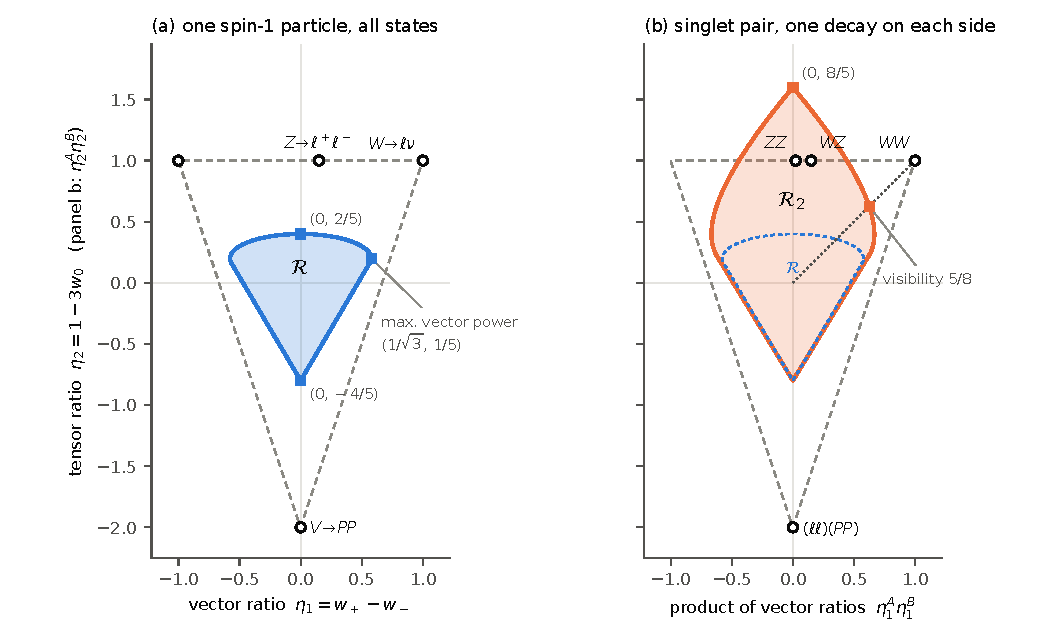
\includegraphics[width=0.78\textwidth]{fig_regions}
\caption{(a) Region $\cR$ of classical spin-$1$ polarimeters in the plane of the vector and tensor ratios (Theorem~\ref{thm:one}). The dashed triangle is the set of all kernels, $w\ge0$; its vertices are the helicity-pure decays. (b) Region $\cR_2$ for a spin-singlet pair with one decay on each side, in the plane of the products of the ratios (Theorem~\ref{thm:onepair}); the dotted line is the isotropic family for two $W\to\ell\nu$ decays, which leaves $\cR_2$ at visibility $5/8$. The dashed outline in (b) repeats $\cR$.}
\label{fig:regions}
\end{figure*}

The set of all kernels is the triangle with vertices $(\eta_1,\eta_2)=(1,1)$, $(-1,1)$, $(0,-2)$, which correspond to $w=(1,0,0)$, $(0,0,1)$, $(0,1,0)$. All three, and the whole edge $\eta_2=1$, lie outside $\cR$: no decay that fixes the helicity along the recorded direction is a classical polarimeter.

\begin{corollary}[Parity-symmetric kernels]
\label{cor:parity}
If $w_+=w_-$, the polarimeter is classical if and only if $\tfrac15\le w_0\le\tfrac35$. For a decay whose direction is distributed as $1+\alpha\cos^2\theta$ about the spin axis of a parent with helicity $\pm1$ this is $-\tfrac12\le\alpha\le\tfrac13$; for a decay into a fermion pair through a vector current, $\alpha=(1-4x)/(1+4x)$ with $x=m_f^2/M^2$, it is $x\ge\tfrac18$.
\end{corollary}

\begin{proof}
$\eta_1=0$ and $-\tfrac45\le\eta_2\le\tfrac25$; $w_0=(1-\alpha)/(3+\alpha)$.
\end{proof}

\begin{remark}[Degenerate kernels]
\label{rem:deg}
For $\eta_1=0\ne\eta_2$ the effects do not separate states that differ only in $\bp$; the criterion of Theorem~\ref{thm:one} remains valid, under both readings, because the end points of the segment $\cR\cap\{\eta_1=0\}$ are realised with $\bp_\psi=\bp_Z=0$ (Appendix~\ref{app:spin1}). For $\eta_2=0$ exactly the situation changes: the data depend on the state through $\bp$ only, $p(\bq)=\frac{1}{4\pi}(1+\tfrac32\eta_1\,\bp\!\cdot\!\bq)$ with $|\bp|\le1$, and Theorem~\ref{thm:half} gives the criterion $|\eta_1|\le\tfrac29$ under reading I; under reading II it is $|\eta_1|\le\tfrac13$. Both are smaller than the limit $\sqrt2/3$ of $\cR$ as $\eta_2\to0$. The set of classical kernels is thus not closed at $\eta_2=0$: for $\eta_2\ne0$, however small, a response function may contain a quadrupole term $\bq^{\T}\tilde A\bq$ of order one, because the effects contain a small quadrupole component to which it is attached linearly; at $\eta_2=0$ no effect carries such a component. A noncontextuality test near $\eta_2=0$ is correspondingly sensitive to the precision with which the equivalences are established \cite{mazurek2016,pusey2018}.
\end{remark}

\subsection{Spin-singlet pair of spin-$1$ particles}

Theorem~\ref{thm:pair}(b) has a counterpart for arbitrary spins. Let particles $A$ and $B$ of spins $j_A$, $j_B$ in a state $\rho$ decay through polarimeters with kernels $w^A$, $w^B$, and let $\cF_{B\to A}$ be the fragment of the states of $A$ steered by outcome sets of $B$, $\omega(\bq_B)=\Tr_B[\rho\,(\openone\otimes E_{w^B}(\bq_B))]$ and their mixtures, with the effects of $A$.

\begin{proposition}
\label{prop:pairpoly}
(i) If $\cF_{B\to A}$ has a noncontextual model, under either reading, then
\begin{equation}
p(\bq_A,\bq_B)=\sum_\lambda r_\lambda(\bq_A)\,s_\lambda(\bq_B)
\label{eq:pairpoly}
\end{equation}
with finitely many nonnegative polynomials $r_\lambda$, $s_\lambda$ on the sphere of degree at most $2j_A$ and $2j_B$.
(ii) If all multipole ratios of both kernels are nonzero and the map $X\mapsto\Tr_B[\rho\,(\openone\otimes X)]$ from Hermitian operators of $B$ to those of $A$ is invertible, the converse holds.
\end{proposition}

\begin{proof}
(i) In a noncontextual model $e(\omega)=\sum_\lambda e(Z_\lambda)g_\lambda(\omega)$ for all effects and states of the fragment. Put $r_\lambda(\bq_A)=\Tr[Z_\lambda E_{w^A}(\bq_A)]$ and $s_\lambda(\bq_B)=g_\lambda(\omega(\bq_B))$. Both are nonnegative, and both are linear functionals of operators whose matrix elements are polynomials of degree $2j$ in the direction. (ii) Under the hypotheses each polynomial of degree $2j_A$ is $\Tr[ZE_{w^A}(\bq_A)]$ for a unique Hermitian $Z$, each polynomial of degree $2j_B$ is $g(\omega(\bq_B))$ for a unique functional $g$, and the states and effects of the fragment span the full operator space, so that Eq.~\eqref{eq:pairpoly} is Eq.~\eqref{eq:simplex}.
\end{proof}

Equation~\eqref{eq:pairpoly} is a local hidden-variable model whose response functions are polynomials of bounded degree; the recorded-outcome model of Remark~\ref{rem:lhv} uses delta functions instead. For spin $1/2$ nonnegative polynomials of degree one are the elements of the Bloch cone and Eq.~\eqref{eq:pairpoly} is Eq.~\eqref{eq:localnc}; Theorem~\ref{thm:pair} shows that the invertibility hypothesis of (ii) is not needed there.

Let $|\Psi_0\rangle=\tfrac{1}{\sqrt3}\sum_m(-1)^{1-m}|m\rangle|{-m}\rangle$ be the state of total spin zero of two spin-$1$ particles and $\rho_v=v|\Psi_0\rangle\langle\Psi_0|+(1-v)\openone/9$ the isotropic family; $\rho_v$ is entangled if and only if $v>\tfrac14$ \cite{horodecki1999}. Each particle decays through a polarimeter, with kernels $w^A$ and $w^B$.

\begin{theorem}
\label{thm:onepair}
Let $\eta_2^A\eta_2^B\ne0$. The decay data of $\rho_v$ have a noncontextual model if and only if
\begin{equation}
\big(v\,\eta_1^A\eta_1^B,\ v\,\eta_2^A\eta_2^B\big)\in\cR_2=\conv\big(\Gamma\cup\Gamma^-\cup\{(0,-\tfrac45)\}\big),
\label{eq:R2}
\end{equation}
where $\Gamma=\{(\tfrac23s(2-s),\tfrac25s^2):0\le s\le2\}$ and $\Gamma^-$ is its mirror image under $\eta_1\to-\eta_1$. The support function is
\begin{equation}
h_{\cR_2}(a,b)=\max\Big\{\max_{0\le s\le2}\big[\tfrac23|a|\,s(2-s)+\tfrac25b\,s^2\big],\ -\tfrac45b\Big\}.
\label{eq:hR2}
\end{equation}
\end{theorem}

The boundary of $\cR_2$ consists of the arcs $\sqrt3-1\le s\le2$ of $\Gamma$ and $\Gamma^-$, which meet at $(0,\tfrac85)$, and of the segments from $\Gamma(\sqrt3-1)$ and its mirror image to $(0,-\tfrac45)$ (Fig.~\ref{fig:regions}b). $\cR_2$ is larger than $\cR$ because the states steered through a decay are images of the coherent cone only, not all states; the functionals $g_\lambda$ then need to be nonnegative on fewer states, and both factors of the model range over $\cQ$ (Appendix~\ref{app:spin1}).

\begin{table}[t]
\caption{Critical visibility $v_c$ of the isotropic spin-$1$ pair state for pairs of decays: the data are contextual if and only if $v>v_c$ (the state is entangled if and only if $v>1/4$). $V\to PP$ is a decay of a vector particle into two pseudoscalars, $V\to\ell\ell$ into a massless lepton pair through a vector current; $A_\ell$ is the leptonic asymmetry parameter of the $Z$.}
\label{tab:pairs}
\begin{ruledtabular}
\begin{tabular}{lcc}
Decays & $(\eta_1^A\eta_1^B,\ \eta_2^A\eta_2^B)$ & $v_c$\\
\hline
$W\to\ell\nu$, $W\to\ell\nu$ & $(\pm1,\ 1)$ & $5/8$\\
$W\to\ell\nu$, $Z\to\ell\ell$ & $(\pm A_\ell,\ 1)$ & none\\
$Z\to\ell\ell$, $Z\to\ell\ell$ & $(A_\ell^2,\ 1)$ & none\\
$V\to\ell\ell$, $V\to\ell\ell$ & $(0,\ 1)$ & none\\
$V\to PP$, $V\to PP$ & $(0,\ 4)$ & $2/5$\\
$V\to PP$, $V\to\ell\ell$ or $W\to\ell\nu$ & $(0,\ -2)$ & $2/5$\\
\end{tabular}
\end{ruledtabular}
\end{table}

\begin{corollary}
\label{cor:vis}
The critical visibilities of Table~\ref{tab:pairs} hold. In particular two ideal $W\to\ell\nu$ decays on a singlet give contextual data if and only if $v>5/8$, and with a $Z\to\ell\ell$ decay on at least one side the data are noncontextual for every $v$.
\end{corollary}

\begin{proof}
The ray $v(1,1)$ meets $\Gamma$ at $s=\tfrac54$, $v=\tfrac58$, on the curved part of the boundary. On the axis $\eta_1=0$, $\cR_2$ is the interval $[-\tfrac45,\tfrac85]$. At $\eta_2^A\eta_2^B=1$ the boundary is at $\eta_1^A\eta_1^B=\tfrac23\sqrt{10}-\tfrac53\approx0.44$, which exceeds $A_\ell=\Ae\pm\AeErr$ \cite{pdg2026}.
\end{proof}

\subsection{Spin $j$}

Let $\xi_{2j}$ denote the largest node of the Gauss--Legendre rule with $j+1$ nodes (the largest zero of the Legendre polynomial $P_{j+1}$) if $j$ is an integer, and the largest node of the Gauss--Radau rule with $j+\tfrac32$ nodes, one of them fixed at $-1$ (the largest zero of $(P_n+P_{n+1})/(1+t)$ with $n=j+\tfrac12$), if $j$ is a half-integer \cite{gautschi2004}.

\begin{theorem}
\label{thm:spinj}
(a) Every classical polarimeter of spin $j$ has vector analysing power $|\kappa_1|\le\xi_{2j}$, under either reading and for any kernel.
(b) The bound is the supremum over classical polarimeters. It is attained by the kernel $D^\star=\frac{d}{4\pi}\int d\bq\,Q^\star(\bq)\,|\bq\rangle\langle\bq|$, where $Q^\star$ is the nonnegative polynomial of degree $2j$ in $q_z$ that vanishes at all nodes except the largest, normalised to $\Tr D^\star=1$, provided all multipole ratios of $D^\star$ are nonzero; this holds for $j\le4$.
(c) For two particles of spins $j_A$, $j_B$ in any state and with any kernels, noncontextual decay data satisfy
\begin{equation}
\big\|\langle\bq_A\bq_B^{\T}\rangle\big\|_1\le\xi_{2j_A}\,\xi_{2j_B},
\label{eq:dipole}
\end{equation}
where $\langle\bq_A\bq_B^{\T}\rangle$ is the $3\times3$ matrix of the moments $\langle q_{A,i}q_{B,k}\rangle$ and $\|\cdot\|_1$ the trace norm. In particular $|\langle\bq_A\!\cdot\!\bq_B\rangle|\le\xi_{2j_A}\xi_{2j_B}$.
\end{theorem}

\begin{proof}[Proof of (a)]
In a noncontextual model $E_w(\bq)=\sum_\lambda G_\lambda\,r_\lambda(\bq)$ with $G_\lambda\ge0$, $\sum_\lambda G_\lambda=\openone$, and $r_\lambda(\bq)=\Tr[Z_\lambda E_w(\bq)]$ a nonnegative polynomial of degree at most $2j$ with $\int d\bq\,r_\lambda=1$ (Remark~\ref{rem:lhv}, Eq.~\eqref{eq:lambda}). Multiplying by $\bq$, integrating and using Eq.~\eqref{eq:firstmoment}, $\kappa_1\bJ/(j+1)=\sum_\lambda G_\lambda\,\bx_\lambda$ with $\bx_\lambda=\int d\bq\,\bq\,r_\lambda(\bq)$. Taking the trace with $\bJ$ and using $\Tr(\bJ\!\cdot\!\bJ)=j(j+1)d$ and $|\bx\!\cdot\!\Tr(G\bJ)|\le j|\bx|\Tr G$ for $G\ge0$ gives $|\kappa_1|\le\max_\lambda|\bx_\lambda|$. Averaging $r_\lambda$ over rotations about $\bx_\lambda$ gives a nonnegative polynomial $f$ of degree at most $2j$ in $t=\bq\!\cdot\!\hat{\bx}_\lambda$ with $\int_{-1}^1f\,dt=1$ and $|\bx_\lambda|=\int_{-1}^1t\,f(t)\,dt$. The quadrature rule named above has positive weights $\omega_k$ and is exact for polynomials of degree $2j+1$, hence for $f$ and $tf$: $\int tf=\sum_k\omega_kt_kf(t_k)\le\xi_{2j}\sum_k\omega_kf(t_k)=\xi_{2j}$.
\end{proof}

\begin{proof}[Proof of (c)]
By Proposition~\ref{prop:pairpoly}(i), $p=\sum_\lambda\pi_\lambda\hat r_\lambda(\bq_A)\hat s_\lambda(\bq_B)$ with weights $\pi_\lambda\ge0$ summing to one and normalised nonnegative polynomials of degree at most $2j_A$, $2j_B$. Their first moments $\bx_\lambda$, $\bm{y}_\lambda$ obey $|\bx_\lambda|\le\xi_{2j_A}$, $|\bm{y}_\lambda|\le\xi_{2j_B}$ by the argument of (a), and $\langle\bq_A\bq_B^{\T}\rangle=\sum_\lambda\pi_\lambda\bx_\lambda\bm{y}_\lambda^{\T}$ has trace norm at most $\sum_\lambda\pi_\lambda|\bx_\lambda||\bm{y}_\lambda|$.
\end{proof}

Part (b) is proved in Appendix~\ref{app:spinj}. Table~\ref{tab:gj} lists the values; $\xi_1=\tfrac13$ and $\xi_2=1/\sqrt3$ reproduce Theorems~\ref{thm:half} and \ref{thm:one}, $\xi_3=(1+\sqrt6)/5$, $\xi_4=\sqrt{3/5}$, and $\xi_{2j}\to1$ for $j\to\infty$: for large spin a classical polarimeter can be almost sharp in its vector part. Part (c) is a test on nine first moments of the data that needs neither the state nor the kernels. For two spin-$1/2$ particles $\langle\bq_A\bq_B^{\T}\rangle=c/9$ and Eq.~\eqref{eq:dipole} is $\|c\|_1\le1$, which is therefore necessary for polarised pairs as well and contains Corollary~\ref{cor:D}. For the spin-$1$ pair state $\rho_v$, $\langle\bq_A\bq_B^{\T}\rangle=-\tfrac16v\,\eta_1^A\eta_1^B\,\openone_3$, and Eq.~\eqref{eq:dipole} reads $v|\eta_1^A\eta_1^B|\le\tfrac23$, the largest abscissa of $\cR_2$: the inequality is tight for $j=\tfrac12$ and $j=1$ in this sense, although it is weaker than Theorems~\ref{thm:pair} and \ref{thm:onepair} away from that direction (it gives $v\le\tfrac23$ instead of $\tfrac58$ for two $W\to\ell\nu$ decays).

\begin{table}[t]
\caption{Largest vector analysing power $\xi_{2j}$ of a classical spin-$j$ polarimeter (Theorem~\ref{thm:spinj}) and the value of the linear programme that maximises the first moment over operators with nonnegative Husimi function (Appendix~\ref{app:numerics}).}
\label{tab:gj}
\begin{ruledtabular}
\begin{tabular}{llll}
$j$ & Quadrature rule & $\xi_{2j}$ & LP value \\
\hline
$1/2$ & Gauss--Radau, 2 nodes & 0.333333 & 0.333333 \\
$1$ & Gauss--Legendre, 2 nodes & 0.577350 & 0.577350 \\
$3/2$ & Gauss--Radau, 3 nodes & 0.689898 & 0.689898 \\
$2$ & Gauss--Legendre, 3 nodes & 0.774597 & 0.774597 \\
$5/2$ & Gauss--Radau, 4 nodes & 0.822824 & 0.822824 \\
$3$ & Gauss--Legendre, 4 nodes & 0.861136 & 0.861137 \\
$7/2$ & Gauss--Radau, 5 nodes & 0.885792 & 0.885792 \\
$4$ & Gauss--Legendre, 5 nodes & 0.906180 & 0.906180 \\
\end{tabular}
\end{ruledtabular}

\end{table}

\section{Applications}
\label{sec:apps}

\subsection{Which decays are classical polarimeters}

\begin{table}[t]
\caption{Analysing powers of spin-$1/2$ decays when only the listed direction is recorded. A polarimeter is classical (noncontextual on all spin states) if and only if $|\kappa|\le1/3$. Leading order, $m_b=0$ and narrow $W$ for the top quark, with $m_t=\mtop\pm\mtopErr$ GeV and $m_W=\mW$ GeV \cite{pdg2026}; $x_0$ is a threshold on the scaled electron energy, Eq.~\eqref{eq:kappacut}.}
\label{tab:kappa}
\begin{ruledtabular}
\begin{tabular}{llc}
Decay & Recorded direction & $|\kappa|$\\
\hline
$t\to b\,\ell^+\nu$, $t\to b\,\bar d u$ & $\ell^+$ or $\bar d$ & $1$\\
 & $b$ (or $W$) & $\kappab$\\
 & $\nu$ or $u$ & $\kappanu\pm\kappanuErr$\\
$\mu\to e\nu\bar\nu$, $\tau\to\ell\nu\bar\nu$ & $e$, $\ell$ (all energies) & $1/3$\\
 & $e$ with $x>x_0>0$ & $>1/3$\\
$\tau\to\pi\nu$ & $\pi$ & $1$\\
$\tau\to\rho\nu$ & $\rho$ & $\taurho$\\
$\Lambda\to p\pi^-$ & $p$ & $0.752$\\
\end{tabular}
\end{ruledtabular}
\end{table}

Table~\ref{tab:kappa} collects analysing powers. Three entries sit at or near the boundary of Theorem~\ref{thm:half}.

\emph{Muon decay.} The direction-only electron asymmetry of the $V\!-\!A$ interaction has $|\kappa|=1/3$ exactly. The four-state model \eqref{eq:tetra} therefore reproduces the distribution $\frac{1}{4\pi}(1\mp\frac13\cos\theta)$ of fully polarised muons for every direction of the polarisation, and no polarimeter with a noncontextual model has a larger analysing power. Any threshold on the electron energy raises $|\kappa|$ above $1/3$, and the energy-resolved decay contains rank-one effects at the end point of the spectrum, so that recording the energy makes the fragment contextual for every $P>1/3$.

\emph{Top quark, $b$-quark direction.} From Eq.~\eqref{eq:kappab}, $|\kappa_b|>1/3$ if and only if $m_t>2m_W=\twomW$~GeV. At the measured masses $|\kappa_b|=\kappab$. The QCD correction computed in Ref.~\cite{brandenburg2002} lowers $|\kappa_b|$ by about $4\%$ at parton level, which does not change the conclusion: the $b$-quark (or $W$) direction is a nonclassical polarimeter.

\emph{Top quark, neutrino or up-type-quark direction.} Equation~\eqref{eq:kappanu} gives $|\kappa_\nu|=\kappanu\pm\kappanuErr$, the uncertainty being that of $m_t$; $|\kappa_\nu|=1/3$ at $\xi=\xistar$, that is, at $m_t=\mtstar$~GeV, $\mtstarPull$ standard deviations above the measured mass (Fig.~\ref{fig:half}b). In Ref.~\cite{brandenburg2002} the $b$-quark mass and the $W$ width together change this analysing power by $1.8\%$ (comparison of Eq.~\eqref{eq:kappanu} with the leading-order value given there) and the QCD correction changes it by $1.4\%$ at parton level and by $2$--$3\%$ for jets; each exceeds the distance of $1\%$ to the boundary. On which side of the boundary this polarimeter lies is therefore not decided by the leading-order formula. The charged-lepton direction is sharp up to a QCD correction of relative size $0.015\,\alpha_s$ \cite{brandenburg2002}; polarimeters built from jets have intermediate analysing powers \cite{brandenburg2002,tweedie2014}.

\begin{figure*}[t]
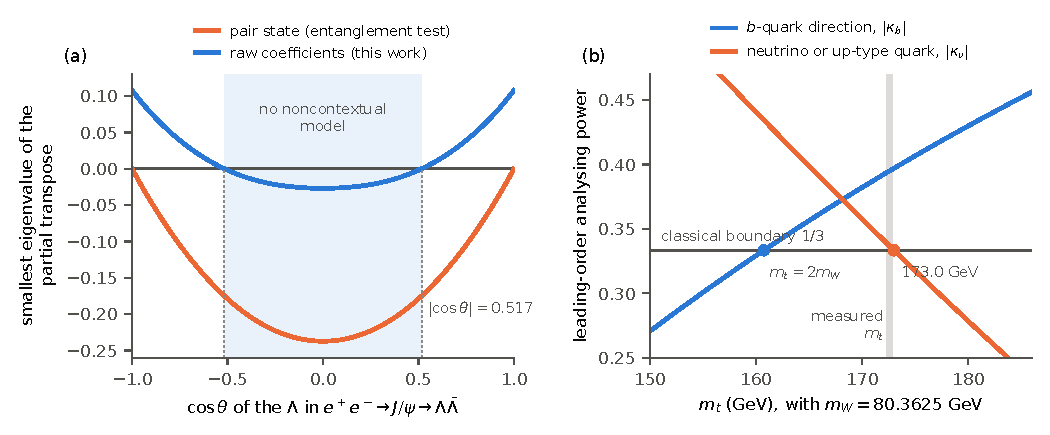
\includegraphics[width=0.86\textwidth]{fig_half}
\caption{(a) Smallest eigenvalue of the partial transpose for $e^+e^-\to J/\psi\to\Lambda\bar\Lambda$ with the BESIII parameters \cite{besiii2022}: of the pair state (the entanglement test) and of $\rhoraw$ built from the raw $p\bar p$ angular coefficients (Theorem~\ref{thm:pair}). The raw data have no noncontextual model in the shaded window. (b) Leading-order analysing powers of the $b$-quark and neutrino directions of top-quark decay against $m_t$; the band is the measured mass \cite{pdg2026}.}
\label{fig:half}
\end{figure*}

\subsection{Top-quark pairs}

ATLAS and CMS measure $D=-3\langle\cos\varphi\rangle$, with $\varphi$ the angle between the two charged-lepton directions, each in the rest frame of its parent top quark. ATLAS reports $D=\DATLAS\pm0.002\,(\text{stat})\pm0.019\,(\text{syst})$ at particle level for $340<m_{t\bar t}<380$~GeV, where the limit $-1/3$ corresponds to $\DATLASbound\pm0.009$ \cite{atlas2024}; CMS reports $D=\DCMS^{+0.026}_{-0.029}$ at parton level in its threshold region \cite{cms2024}. By Corollary~\ref{cor:D} noncontextual lepton-direction data satisfy $|D|\le1/3$, the same number as the separability limit for $|\kappa_\ell|=1$. The measurements therefore exclude a noncontextual model of the lepton-direction data at the significance obtained for entanglement: $\zCMS$ standard deviations for CMS, and $\zATLAS$ for ATLAS if the quoted uncertainties of the measurement and of the folded limit are added in quadrature (ATLAS states more than five).

Three points distinguish this reading from the entanglement reading of the same numbers. First, the bound $|D|\le1/3$ is derived for the raw coefficients and needs no value of the analysing power; the entanglement inference divides by $\kappa_\ell\bar\kappa_\ell$. Second, the statement concerns the data rather than the state: the local hidden-variable model that always exists for these data (Remark~\ref{rem:lhv}) is contextual, and every local model whose response functions are linear in the effects is excluded. Third, the two criteria separate for other decay channels. For unpolarised pairs $\|c\|_1=|\kappa_A\kappa_B|\,\|C\|_1\le3|\kappa_A\kappa_B|$. With the $b$-quark direction on both sides $\kappa_b^2=\kbsq$, so $\|c\|_1<1$ and the data are noncontextual for every spin state, entangled or not; with a neutrino or up-type-quark direction on one side the same holds if $|\kappa_\nu|\le1/3$ (Corollary~\ref{cor:weak}); with a charged lepton on one side and the $b$ quark on the other, contextuality requires $\|C\|_1>1/|\kappa_b|=\Cneed$. Only channels with the charged lepton or the down-type quark on both sides test contextuality at the level at which entanglement is tested.

The statements above are subject to the same qualifications as the entanglement measurements: the coefficient $D$ refers to the distribution unfolded to the full phase space, the limit at particle level is obtained from simulation, and the events of the selected region are averaged in an event-dependent basis. The last point does not affect Corollary~\ref{cor:D}: the trace of $c$ is basis independent, and the set of noncontextual coefficient matrices is convex.

\subsection{Hyperon pairs}

For $e^+e^-\to J/\psi\to\Lambda\bar\Lambda\to p\pi^-\bar p\pi^+$ the joint angular distribution is known in closed form \cite{faldt2017}. In the frame of Ref.~\cite{faldt2017}, with $\theta$ the production angle of the $\Lambda$ and $N=1+\alpha_\psi\cos^2\theta$, the pair state has polarisations $P_y=\sqrt{1-\alpha_\psi^2}\,\sin\Delta\Phi\,\sin\theta\cos\theta/N$ for both hyperons and correlations $C_{xx}=\sin^2\theta/N$, $C_{yy}=-\alpha_\psi\sin^2\theta/N$, $C_{zz}=(\alpha_\psi+\cos^2\theta)/N$, $C_{xz}=C_{zx}=\sqrt{1-\alpha_\psi^2}\,\cos\Delta\Phi\,\sin\theta\cos\theta/N$. The raw coefficients are $\ba=\alpha_-P_y\hat{\bm y}$, $\bb=\alpha_+P_y\hat{\bm y}$, $c=\alpha_-\alpha_+C$. With the BESIII values $\alpha_\psi=\alphapsi$, $\Delta\Phi=\dphi$, $\alpha_-=\alpham$, $\alpha_+=\alphap$ \cite{besiii2022}:

(i) At $\theta=90^\circ$ the pair is unpolarised and $\|c\|_1=|\alpha_-\alpha_+|(1+2\alpha_\psi)=\cnorm$ ($\cnormAvg\pm\cnormErr$ with the average decay parameter and uncorrelated uncertainties), above the bound of Corollary~\ref{cor:tstate}.

(ii) $\rhoraw$ fails the test of Theorem~\ref{thm:pair} for $|\cos\theta|<\cosc$ (between $\coscLo$ and $\coscHi$ when the parameters are shifted by their uncertainties), a window containing $\fracEvents\%$ of the events. Outside the window the $p\bar p$ angular data have a noncontextual model, although the $\Lambda\bar\Lambda$ state is entangled at every angle except $\cos\theta=\pm1$ (Fig.~\ref{fig:half}a). The reason is $|\alpha_-\alpha_+|=\alphaprod$: by Corollary~\ref{cor:ent} the decay data of an entangled state need not be contextual.

(iii) For $J/\psi\to\Sigma^+\bar\Sigma^-$ the decay parameters of $\Sigma^+\to p\pi^0$ are close to $\mp1$ \cite{besiii2020sigma}, the polarimeters are almost sharp, and the two tests nearly coincide; at $90^\circ$, $\|c\|_1=\cnormSigma\pm\cnormSigmaErr$.

These statements are conditional on the fitted form: they say that the distribution which BESIII has fitted has no noncontextual model in the window. A direct test would measure the fifteen raw moments $\langle q_{A,i}\rangle$, $\langle q_{B,k}\rangle$, $\langle q_{A,i}q_{B,k}\rangle$ in bins of $\cos\theta$, without the helicity-formalism parametrisation, and evaluate $\rhoraw$; Eq.~\eqref{eq:dipole} needs the nine correlation moments only. Bell-type tests with hyperon pairs \cite{tornqvist1981,besiii2025} use decay-angle data of the same kind under additional assumptions about the decay.

\subsection{Vector bosons and vector mesons}

\emph{One particle.} The lepton direction of $W\to\ell\nu$ has the kernel $(\eta_1,\eta_2)=(\pm1,1)$, that of $Z\to\ell^+\ell^-$ has $(A_\ell,1)$, a decay into two pseudoscalars has $(0,-2)$ and a decay into a massless lepton pair through a vector current $(0,1)$. All lie outside $\cR$ (Fig.~\ref{fig:regions}a). For the baryon direction in $J/\psi\to B\bar B$, parity conservation gives $\eta_1=0$ and the production-angle parameter $\alpha_\psi$ fixes $w_0=(1-\alpha_\psi)/(3+\alpha_\psi)$. By Corollary~\ref{cor:parity}, $J/\psi\to\Lambda\bar\Lambda$ ($w_0=\wzeroLambda<\tfrac15$) is a nonclassical polarimeter of the $J/\psi$ spin; $J/\psi\to\Sigma^+\bar\Sigma^-$, with $\alpha_\psi=\alphaSigma\pm\alphaSigmaErr$ \cite{besiii2020sigma}, has $w_0=\wzeroSigma\pm\wzeroSigmaErr$, $\zSigma$ standard deviations above the upper boundary $\tfrac35$; and $\psi(2S)\to\tau^+\tau^-$, with $x=m_\tau^2/M^2=\xtau\ge\tfrac18$ \cite{pdg2024}, is a classical polarimeter. These are statements about the measurement on all spin-$1$ states; in $e^+e^-$ annihilation only the mixture of helicities $\pm1$ along the beam is prepared.

\emph{Pairs.} Table~\ref{tab:pairs} gives the visibilities above which the decay data of an isotropic spin-$1$ pair are contextual. The values $5/8$ and $2/5$ are well above the entanglement threshold $1/4$, and pairs with a $Z\to\ell\ell$ decay give noncontextual data at every visibility, because $A_\ell$ is small. Vector-boson pairs from Higgs-boson decays or from diboson production are not in the isotropic family in general; for them Theorem~\ref{thm:onepair} does not apply, but Eq.~\eqref{eq:dipole} does: for any state of two spin-$1$ particles, noncontextual data obey $|\langle\bq_A\!\cdot\!\bq_B\rangle|\le1/3$.

\section{The result as a three-layer concept graph}
\label{sec:graph}

\begin{figure*}[t]
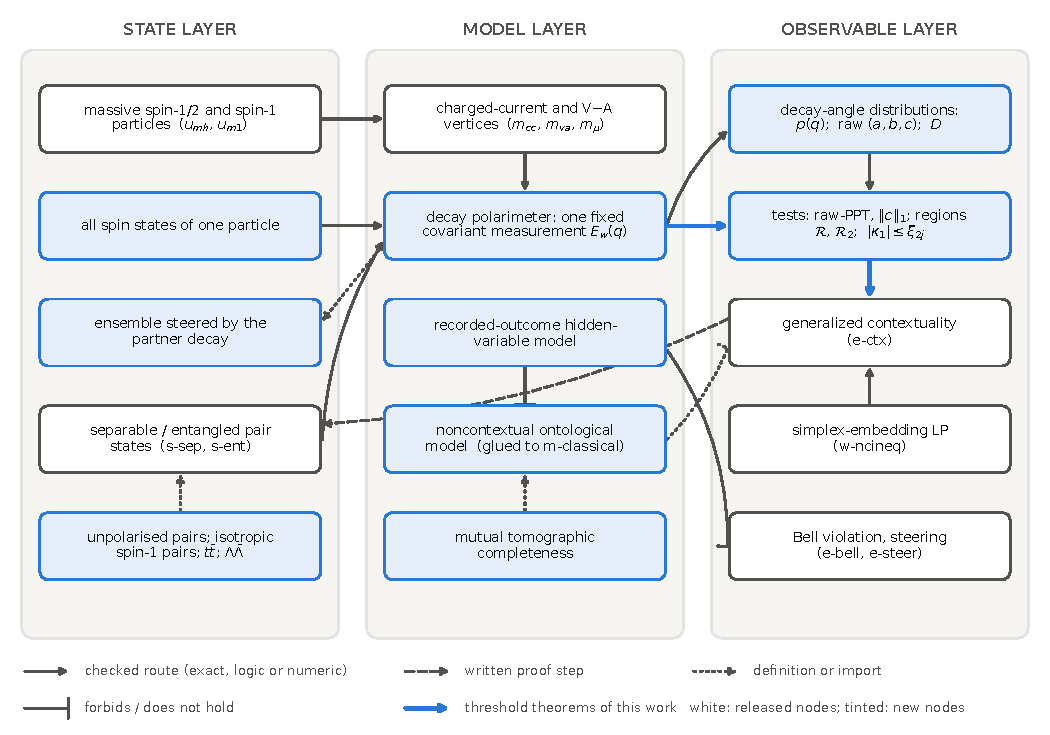
\includegraphics[width=0.86\textwidth]{fig_network}
\caption{The routes of this paper in the three-layer concept graph (condensed: several nodes and routes are merged in each box and arrow; the full list is in Appendix~\ref{app:catalogue}). State layer: what is prepared. Model layer: what assigns probabilities. Observable layer: what is recorded or decided. White boxes are nodes of the released graphs \cite{genhep,gengpt}, tinted boxes are new. The thick arrows are the threshold theorems; the bar-ended line records that the recorded-outcome model forbids Bell violation and steering while it is not a noncontextual model.}
\label{fig:network}
\end{figure*}

The statements of Secs.~\ref{sec:setting}--\ref{sec:apps} are encoded as a graph with three layers. \emph{State} nodes are things that are prepared: particles as representations, sets of spin states, steered ensembles, separable and entangled pair states. \emph{Model} nodes assign probabilities: interaction terms, the Born rule, the decay polarimeter, hidden-variable and ontological models, and assumptions such as tomographic completeness. \emph{Observable} nodes are what is recorded or decided: angular distributions and their coefficients, tests, and effects such as generalized contextuality or Bell violation. There are \nNodes\ nodes (\nS\ state, \nM\ model, \nO\ observable); \nReleased\ keep the identifiers of the released graph of particle physics \cite{genhep} and of the Nonclassicality Network \cite{gengpt} (with links to the resource-theory graph \cite{genqrt}), and \nNew\ are new (Appendix~\ref{app:catalogue}).

A \emph{route} is a statement with input nodes, a target node, a relation (derives, implies, equivalent, forbids, witness, defines) and a grade:
\emph{exact}, an identity or equivalence checked in exact arithmetic by computer algebra \cite{sympy2017};
\emph{logic}, a statement whose negation is shown unsatisfiable by an SMT solver \cite{z3};
\emph{numeric}, a floating-point computation with a stated tolerance \cite{scipy,highs,cvxpy,clarabel}, or the reading of a recorded long run;
\emph{import}, a statement cited from the literature;
\emph{definition}; and
\emph{written}, a proof given in this paper that no program has checked.
Of the \nRoutes\ routes, \nChecked\ carry certificates that are executed (\nExact\ exact, \nLogic\ logic, \nNumeric\ numeric, and \nImportChecked\ import with a consistency check), \nImported\ are imports, \nDefinitions\ are definitions and \nWritten\ are written proofs. No certificate fails.

Each headline claim lists the routes it rests on, and its verdict is the weakest status among them (Table~\ref{tab:claims}). Two claims are verified by executed certificates alone; the theorems are verified modulo the written proofs and the imported simplex-embedding lemma.

\begin{table}[t]
\caption{Headline claims, the routes they rest on, and the verdict of the closure. C1: the decay as a fixed covariant measurement and the $V\!-\!A$ kernels. C2: single-setting data admit a recorded-outcome model that is not noncontextual. C3--C4: Theorems~\ref{thm:half}, \ref{thm:pair}. C5--C6: Theorems~\ref{thm:one}, \ref{thm:onepair}. C7: Theorem~\ref{thm:spinj}. C8--C11: applications to top-quark pairs, hyperon pairs, top-quark polarimeters and vector mesons.}
\label{tab:claims}
\begin{ruledtabular}
\begin{tabular}{lp{0.50\columnwidth}p{0.30\columnwidth}}
Claim & Routes & Verdict \\
\hline
C1 & DV1, DV2, DV3, DV6 & verified modulo written proofs \\
C2 & FW2, FW3, FW4, FW5 & verified \\
C3 & FW1, H1, H2 & verified modulo imports \\
C4 & FW1, DV9, H3, H4, H12, H5, H6, H7, H10 & verified modulo imports and written proofs \\
C5 & FW1, FW6, DV7, V1, V2, V3, V4, V5, V6, P5 & verified modulo imports and written proofs \\
C6 & FW1, FW6, DV7, V1, V2, P1, P2, P3, P6, P4, P5 & verified modulo imports and written proofs \\
C7 & FW1, FW6, G1, G2, G3, G4, G5, G6, G7 & verified modulo imports and written proofs \\
C8 & H6, A1, A2 & verified modulo imports \\
C9 & H3, H4, DV9, A3, A4 & verified modulo imports and written proofs \\
C10 & H1, H2, DV4, DV5 & verified \\
C11 & V3, V5, A7, A8 & verified modulo imports and written proofs \\
\end{tabular}
\end{ruledtabular}

\end{table}

Three further checks are part of the encoding. (i) \emph{Negative controls}: \nControls\ errors are planted in accepted statements (a threshold $1/2$ instead of $1/3$; the opposite sign of the spin vector in Eq.~\eqref{eq:trace}; the Frobenius norm instead of the trace norm in Corollary~\ref{cor:tstate}; a shifted ellipse; a different apex; a wrong coefficient in Eq.~\eqref{eq:m12}; a Euclidean projector in Lemma~\ref{lem:range}; and others), and the corresponding check must reject each; \nControlsRejected\ are rejected. (ii) \emph{Lint}: every observable node is reached by a route from the model layer, every effect node has a witness, and no node is unused. (iii) \emph{Scope separation}: the route ``the recorded-outcome model forbids Bell violation'' and the route ``the recorded-outcome model is not a noncontextual model'' must both be present and certified, so that the conclusion ``no Bell test, yet contextuality is testable'' cannot arise from mixing the two notions.

What the graph contributed is the following. The question was read off as a missing connection between two released graphs. Every theorem is a path across the layers: for Theorem~\ref{thm:pair}, from the entangled-state node through the polarimeter node to the joint distribution, the raw test and the contextuality node, with one back-edge from the model layer to the state layer, since the decay of the partner defines the steered ensemble. Two released edges of the Nonclassicality Network reappear with the measurement fixed: simplex embedding as the definition of classicality, and contextuality as a precondition of entanglement \cite{plavala2024}, which becomes a strict implication (Corollary~\ref{cor:ent}). Finally, the grades separate what was computed from what was proved by hand and from what was cited; this separation is the content of the verdicts and it is not a substitute for a formal proof of the written steps.

\section{Discussion}
\label{sec:discussion}

\emph{Assumptions.} The operational equivalences used here follow from the quantum description of the decay: a parent of definite spin $j$, rotation covariance, and hence angular distributions of degree at most $2j$. Under reading I they are properties of the data and can be checked on the data, for instance by the absence of higher harmonics; but an equivalence is a statement about all preparations, and only those of the fragment can be examined. This is the tomographic-completeness assumption common to noncontextuality tests \cite{mazurek2016,pusey2018}. The theorems also assume full angular acceptance; selections that depend on the recorded directions break covariance and must be removed by unfolding, as in the entanglement analyses.

\emph{What is excluded.} A failure of noncontextuality is not a loophole-free exclusion of local hidden variables: the recorded-outcome model always exists. What is excluded is every hidden-variable account in which the response to a set of outcomes depends only on the effect that the set defines, equivalently every local model with polynomial response functions of degree $2j$ [Eq.~\eqref{eq:pairpoly}]. Whether this is the appropriate notion of classicality for collider data is a matter of interpretation. In its favour: it is the notion equivalent to simplex embedding and to nonnegative quasiprobability representations \cite{schmid2021,spekkens2008}, it reduces to separability when all local measurements are available \cite{plavala2024}, and for decays it gives conditions on measured coefficients with thresholds that are neither trivial nor identical to those of entanglement.

\emph{Relation to entanglement measurements.} For decay data, contextuality implies entanglement and is strictly stronger unless both analysing powers are maximal. It is tested on raw angular coefficients and needs large analysing powers on both sides: $|\kappa|>1/3$ for spin $1/2$, kernels outside $\cR$ for spin $1$. The three examples of Sec.~\ref{sec:apps} show the three possibilities: for top-quark pairs with two charged leptons the tests coincide; for $J/\psi\to\Lambda\bar\Lambda$ the state is entangled everywhere and the data are contextual in a window; for pairs analysed through $b$ quarks, or through a $Z\to\ell\ell$ decay of a spin-$1$ partner, the data are noncontextual whatever the state.

\emph{Open problems.}
(1) Spin-$1$ pairs outside the isotropic family, in particular $H\to WW^*$ and $H\to ZZ^*$. By Proposition~\ref{prop:pairpoly} the question is whether a polynomial of bidegree $(2,2)$ lies in the cone generated by products of nonnegative quadratic polynomials on two spheres; Lemma~\ref{lem:sos} describes one factor, and the linear programmes of Appendix~\ref{app:numerics} decide instances.
(2) The exact region of classical kernels for $j\ge\tfrac32$; Theorem~\ref{thm:spinj} gives its extent in the vector direction only.
(3) Whether the extremal kernel $D^\star$ has nonzero multipole ratios for all $j$, which would make the bound of Theorem~\ref{thm:spinj} a maximum for all $j$.
(4) Exactly degenerate kernels (Remark~\ref{rem:deg}) and, with them, the robustness of the criteria to imperfect equivalences and finite statistics; noise-robust inequalities follow from the duals of the linear programmes \cite{selby2024lp,kunjwal2019}, and the witnesses of Corollary~\ref{cor:D} and Eq.~\eqref{eq:dipole} are the simplest examples.
(5) Decays with recorded energies and cascades such as $\Xi\to\Lambda\pi\to p\pi\pi$, where the polarimeter has more than one stage.


\begin{acknowledgments}
\emph{Use of an AI system.} The derivations, the code and the text were produced in a dialogue between the author and an AI system (Claude, Anthropic), which also carried out the literature searches and wrote the certificates. Statements graded ``written'' in Appendix~\ref{app:catalogue} are proofs given in this paper that no program has checked; no independent reviewer, human or machine, has examined them. The author is responsible for the content.

\emph{Data and code.} The node, route and claim encoding, all certificates, the recorded numerical runs, the negative controls and the scripts that generate every number, table and figure of this paper are in the accompanying archive (\texttt{run\_all.py} reproduces the summary in \runSeconds~s on two cores; the recorded linear programmes take several minutes each). The released graphs from which \nReleased\ nodes are taken are Refs.~\cite{genhep,gengpt,genqrt}.
\end{acknowledgments}

\appendix
\section{Proof of Lemma~\ref{lem:simplex}}
\label{app:lemma1}

The statement is that of Refs.~\cite{schmid2021,selby2024lp} for the fragment at hand; we recall the argument. Let a noncontextual model be given. In an ontological model a mixture of preparations is represented by the mixture of their distributions, and by noncontextuality $\mu(\lambda|\cdot)$ depends on the preparation only through the vector $\omega\in V$. A convex-linear function on $\Omega$ extends uniquely to a linear functional $g_\lambda$ on $V=\operatorname{span}\Omega$. Likewise $r(\cdot|\lambda)$ is convex-linear, additive under coarse-graining, and depends on an effect only through its restriction to $V$; because the effects separate the points of $V$, their restrictions span the dual of $V$, and $r(e|\lambda)=e(Z_\lambda)$ for a unique $Z_\lambda\in V$. Reproduction of the statistics, $e(\omega)=\sum_\lambda e(Z_\lambda)g_\lambda(\omega)$ for all $e$ and $\omega$, is $\sum_\lambda Z_\lambda g_\lambda(\cdot)=\mathrm{id}_V$, and nonnegativity of $\mu$ and $r$ gives the inequalities of Eq.~\eqref{eq:simplex}. Conversely, given Eq.~\eqref{eq:simplex}, terms with $u(Z_\lambda)=0$ have $e(Z_\lambda)=0$ for every effect (since $0\le e(Z_\lambda)\le u(Z_\lambda)$) and can be dropped. Applying $u$ to the decomposition of the identity gives $\sum_\lambda u(Z_\lambda)g_\lambda=u$ on $V$, so that $\mu(\lambda|\omega)=u(Z_\lambda)g_\lambda(\omega)$ is a probability distribution and $r(e|\lambda)=e(Z_\lambda)/u(Z_\lambda)\in[0,1]$ with $r(u|\lambda)=1$. Both depend on states and effects only through their vectors, so the model is noncontextual. That a finite ontic set suffices is shown in Ref.~\cite{schmid2021}. \hfill$\square$

When the effects do not separate the points of $V$ (degenerate kernels), states that differ by an element of $N=\{v\in V:e(v)=0\ \forall e\in\cE\}$ are equivalent under reading I and the lemma applies to $V/N$; under reading II the $g_\lambda$ are functionals on the full operator space and the $Z_\lambda$ functionals on the span of the effects. Both cases are treated where they occur (Remark~\ref{rem:deg}).

\section{Charged-current kernels}
\label{app:va}

Equation~\eqref{eq:trace} is a polynomial identity in the components of the momenta and of the spin vector; route DV1 verifies it with explicit Dirac matrices. For the fermion of the second current, the two unobserved massless momenta are integrated with
\begin{equation}
\int\!\frac{d^3p_2}{2E_2}\frac{d^3p_4}{2E_4}\,\delta^4(Q-p_2-p_4)\,p_2^\alpha p_4^\beta=\frac{\pi}{24}\big(g^{\alpha\beta}Q^2+2Q^\alpha Q^\beta\big),
\end{equation}
$Q=p_1-p_3$. In the rest frame, with $x=2E_3/m$ and $c=\hat{\bm s}\!\cdot\!\bq_3$, one has $Q^2=m^2(1-x)$, $p_3\!\cdot\!(p_1-ms)=\tfrac12m^2x(1+c)$, $Q\!\cdot\!p_3=\tfrac12m^2x$ and $Q\!\cdot\!(p_1-ms)=m^2(1-\tfrac x2-\tfrac x2c)$, so that $p_{3\alpha}(p_1-ms)_\beta(g^{\alpha\beta}Q^2+2Q^\alpha Q^\beta)=\tfrac12m^4x\,[(3-2x)-(2x-1)c]$; with the phase-space factor $x\,dx\,d\bq$ this is Eq.~\eqref{eq:michel}, and Eq.~\eqref{eq:kappacut} follows by integration (route DV3).

For $t\to bW$ with $m_b=0$ the $b$ quark has helicity $-\tfrac12$, so a $W$ of helicity $0$ or $-1$ along its direction $\bn$ carries the top spin projection $+\tfrac12$ or $-\tfrac12$ along $\bn$. The kernel of the $W$ direction is therefore $(w_{+},w_{-})=(F_0,F_-)$ with the helicity fractions $F_0=\xi/(\xi+2)$, $F_-=2/(\xi+2)$, and the $b$ quark, emitted opposite, has $\kappa_b=-(F_0-F_-)$, Eq.~\eqref{eq:kappab} (route DV4). Equation~\eqref{eq:kappanu} results from integrating Eq.~\eqref{eq:trace} with a narrow $W$ over the variables other than the neutrino direction; route DV5 checks it against a direct numerical quadrature of Eq.~\eqref{eq:trace}, which also returns $\kappa_\ell=1$ and Eq.~\eqref{eq:kappab}. The entries for $\tau$ decays in Table~\ref{tab:kappa} are those of Ref.~\cite{tsai1971}; for $\tau\to\rho\nu$ with only the $\rho$ direction recorded, $\kappa=(m_\tau^2-2m_\rho^2)/(m_\tau^2+2m_\rho^2)$, which is the same helicity counting with $m_t\to m_\tau$, $m_W\to m_\rho$ \cite{pdg2024}.

\section{Range lemma}
\label{app:range}

\begin{lemma}
\label{lem:range}
Let $W\subset\mathbb{R}^4$ be a linear subspace that contains an interior point $u$ of the Bloch cone $\cK$. There is a linear projection $P$ onto $W$ with $P\cK\subset\cK$.
\end{lemma}

\begin{proof}
$\cK$ is the forward light cone. Let $L$ be the Lorentz boost with $Lu\propto e_0=(1,\bm{0})$; $L\cK=\cK$. The subspace $LW$ contains $e_0$, hence $LW=\mathbb{R}e_0\oplus(\{0\}\times S)$ with $S\subset\mathbb{R}^3$. Let $\Pi=1\oplus\Pi_S$ with $\Pi_S$ the orthogonal projector onto $S$. Then $\Pi$ is a projection onto $LW$, and $\Pi\cK\subset\cK$ because $|\Pi_S\bx|\le|\bx|\le t$. Put $P=L^{-1}\Pi L$.
\end{proof}

In Theorem~\ref{thm:pair}, $\operatorname{range}\Rraw$ contains $\Rraw e_0=(1,\ba)$ and $\operatorname{range}\Rraw^{\T}$ contains $(1,\bb)$. With $P_A$, $P_B$ the projections of the lemma, $P_A\Rraw=\Rraw$ and $P_B\Rraw^{\T}=\Rraw^{\T}$, so that a decomposition $\Rraw=\sum_\lambda z_\lambda h_\lambda^{\T}$ with $z_\lambda,h_\lambda\in\cK$ yields $\Rraw=P_A\Rraw P_B^{\T}=\sum_\lambda(P_Az_\lambda)(P_Bh_\lambda)^{\T}$ with factors in $\cK\cap\operatorname{range}\Rraw$ and $\cK\cap\operatorname{range}\Rraw^{\T}$. Route H12 checks the construction on random singular matrices whose given decomposition violates Eq.~\eqref{eq:rangecond}. A Euclidean orthogonal projector does not have the property (negative control k15).

\section{Proof of Proposition~\ref{prop:cov}}
\label{app:cov}

Since all $\eta_l\ne0$, the effects $E_w(\bq)$ span the Hermitian operators, and Lemma~\ref{lem:simplex} applies with $V$ the space of Hermitian operators: the polarimeter is classical if and only if there are $G_\lambda\ge0$ and Hermitian $Z_\lambda$ with $X=\sum_\lambda Z_\lambda\Tr[G_\lambda X]$ for all $X$ and $\Tr[Z_\lambda E_w(\bq)]\ge0$. By Eq.~\eqref{eq:lambda} the last condition says that $Z'_\lambda=\Lambda_\eta Z_\lambda$ has a nonnegative Husimi function. Applying $\Lambda_\eta$, the conditions become
\begin{equation}
\Lambda_\eta=\sum_\lambda|Z'_\lambda\rangle\!\rangle\langle\!\langle G_\lambda|,\qquad G_\lambda\ge0,\quad Q_{Z'_\lambda}\ge0 ,
\label{eq:lamdec}
\end{equation}
where $|Z\rangle\!\rangle\langle\!\langle G|$ denotes the map $X\mapsto Z\Tr[GX]$; conversely Eq.~\eqref{eq:lamdec} gives $Z_\lambda=\Lambda_\eta^{-1}Z'_\lambda$. Both sides can be averaged over rotations acting by conjugation. The operator space carries each rank $l=0,\dots,2j$ once, so by Schur's lemma the average of $|Z'\rangle\!\rangle\langle\!\langle G|$ is $\sum_l(2l+1)^{-1}\Tr(\Pi_l[G]\Pi_l[Z'])\,\Pi_l$. Decomposing each $G_\lambda$ into rank-one terms and normalising $\Tr Z'_\lambda=1$ (the rank-$0$ component gives $\sum_\lambda\Tr G_\lambda=d$), Eq.~\eqref{eq:lamdec} implies $\eta_l=\sum_k\pi_km_l(\psi_k,Z'_k)$ with weights $\pi_k\ge0$ summing to one and $m_l$ as in Eq.~\eqref{eq:ml}. Conversely, if $\eta=\sum_k\pi_km(\psi_k,Z'_k)$, then $\Lambda_\eta=\sum_k\pi_kd\int\!dU\,|UZ'_kU^\dagger\rangle\!\rangle\langle\!\langle U\psi_k\psi_k^\dagger U^\dagger|$. The integral is a point of the convex hull of a compact set in a finite-dimensional space, hence a finite convex combination of its elements (Carath\'eodory), which is Eq.~\eqref{eq:lamdec}. \hfill$\square$

For $j=1$ the Haar average can be replaced by the average over the $60$ rotations of the icosahedral group: maps on the nine-dimensional operator space decompose into tensor ranks up to four, and the icosahedral group has no invariant of rank one to five \cite{klein1956}. This gives the finite models of Appendix~\ref{app:finite}.

\section{Spin $1$: proofs}
\label{app:spin1}

\subsection{Nonnegative quadratic functions on the sphere}

Let $J=\operatorname{diag}(1,-1,-1,-1)$.

\begin{lemma}
\label{lem:sos}
(a) A real symmetric $4\times4$ matrix satisfies $M\ge0$ and $\Tr(MJ)=0$ if and only if $M=\sum_kc_k(1,\bq_k)(1,\bq_k)^{\T}$ with $c_k\ge0$ and unit vectors $\bq_k$; that is, if and only if its entries are the moments of order at most two of a positive measure on the sphere.
(b) $F(\bq)=f_0+\bm{f}\!\cdot\!\bq+\bq^{\T}F_2\bq$ is nonnegative on the unit sphere if and only if, for some real $\mu$,
\begin{equation}
\begin{pmatrix}f_0+\mu&\tfrac12\bm{f}^{\T}\\ \tfrac12\bm{f}&F_2-\mu\openone_3\end{pmatrix}\ge0 ,
\label{eq:pencil}
\end{equation}
that is, if and only if $F$ coincides on the sphere with a sum of squares of affine functions.
\end{lemma}

\begin{proof}
(a) ``If'' is immediate. For ``only if'' write $M=BB^{\T}$ with columns $b_k$. The symmetric matrix $N=B^{\T}JB$ has $\Tr N=\Tr(JM)=0$. A real symmetric matrix of trace zero has zero diagonal in a suitable orthonormal basis: there is a unit vector $x$ with $x^{\T}Nx=0$, because the quadratic form takes both signs or vanishes, and one proceeds by induction on the orthogonal complement. With the corresponding orthogonal matrix $O$, the columns $u_k$ of $BO$ satisfy $u_k^{\T}Ju_k=0$ and $\sum_ku_ku_k^{\T}=M$; a lightlike vector is $\pm\sqrt{c}\,(1,\bq)$.
(b) ``If'': on the sphere the terms in $\mu$ cancel. ``Only if'': the set $\mathcal{P}$ of matrices $P+\mu J$ with $P\ge0$ is a convex cone, and it is closed: if $P_n+\mu_nJ$ converges and $|\mu_n|\to\infty$, then $P_n/|\mu_n|\to\mp J$, which is not positive. Let $M_F$ be the matrix \eqref{eq:pencil} at $\mu=0$, so that $F(\bq)=(1,\bq)M_F(1,\bq)^{\T}$. If $M_F$ were not in $\mathcal{P}$, a separating matrix $M$ would satisfy $\Tr(MP)\ge0$ for all $P\ge0$, $\Tr(MJ)=0$ and $\Tr(MM_F)<0$. By (a), $\Tr(MM_F)=\sum_kc_kF(\bq_k)\ge0$, a contradiction.
\end{proof}

These are the forms of the $S$-lemma needed here \cite{sturm2003,polik2007}; route V2 checks the construction in (a) on random matrices. By (b), every element of $\cQ$ is a convex combination of the operators $Z_{\tau,\bn}^{\pm}$ for which the left-hand side of Eq.~\eqref{eq:Q1} is the square $(\pm\sqrt{(2-\tau)/3}+\sqrt\tau\,\bn\!\cdot\!\bq)^2$, $0\le\tau\le2$; they have
\begin{equation}
\bp=\pm2\sqrt{\tau(2-\tau)/3}\;\bn,\qquad A=\tau\,(\bn\bn^{\T}-\tfrac13\openone_3).
\label{eq:squares}
\end{equation}

\subsection{Proof of Theorem~\ref{thm:one}}

By Proposition~\ref{prop:cov} the classical kernels with $\eta_1\eta_2\ne0$ are those in the convex hull $\cR$ of the points \eqref{eq:m12}. $\cR$ is compact, so it is determined by its support function $h(a,b)=\max[a\,m_1+b\,m_2]$.

\emph{Upper bound.} Fix $\psi=\psi_\alpha$ and write $am_1+bm_2=\bz\!\cdot\!\bp_Z+\Tr(\mathsf{Z}A_Z)$ with $\bz=\tfrac a2\bp_\psi$ and $\mathsf{Z}=\tfrac{3b}{5}A_\psi$. If $t$ is such that
\begin{equation}
M(t)=\begin{pmatrix}t&-\bz^{\T}\\-\bz&\tfrac t3\openone_3-\mathsf{Z}\end{pmatrix}\ge0 ,
\label{eq:Mt}
\end{equation}
then, since $\Tr(M(t)J)=0$, Lemma~\ref{lem:sos}(a) gives $M(t)=\sum_kc_k(1,\bq_k)(1,\bq_k)^{\T}$, and for every $(\bp_Z,A_Z)\in\cQ$
\begin{equation}
0\le\sum_kc_k\big[\tfrac23+\bp_Z\!\cdot\!\bq_k+\bq_k^{\T}A_Z\bq_k\big]=\tfrac23t-\bz\!\cdot\!\bp_Z-\Tr(\mathsf{Z}A_Z).
\end{equation}
Hence $am_1+bm_2\le\tfrac23t$. For $\psi_\alpha$ the matrix \eqref{eq:Mt} is block diagonal with entries $\tfrac t3-\tfrac b5+\tfrac{3b}{5}\cos^2\!\alpha$, $\tfrac t3-\tfrac b5+\tfrac{3b}{5}\sin^2\!\alpha$ and the $2\times2$ block $\big(\begin{smallmatrix}t&-\frac a2\sin2\alpha\\-\frac a2\sin2\alpha&\frac t3-\frac b5\end{smallmatrix}\big)$. For $b\ge0$ the block is binding and the smallest admissible $t$ gives $\tfrac23t=\tfrac b5+(\tfrac{b^2}{25}+\tfrac{a^2}{3}\sin^22\alpha)^{1/2}$, largest at $\alpha=\pi/4$. For $b<0$, $t$ must exceed both $t_1(\alpha)=\tfrac{3|b|}{5}(3\cos^2\!\alpha-1)$, which decreases on $[0,\pi/4]$, and the root $t_2(\alpha)$ of the block condition, which increases; hence $\tfrac23t\le\max\{\tfrac23t_1(0),\tfrac23t_2(\pi/4)\}$. In both cases $h(a,b)\le h_{\cR}(a,b)$ of Eq.~\eqref{eq:hR}.

\emph{Attainment.} The first entry of Eq.~\eqref{eq:hR} is the support function of the ellipse, whose points $(\pm\sqrt{\tau(2-\tau)/3},\tau/5)$ are $m(\psi_{\pi/4},Z^{\pm}_{\tau,\bm{e}_z})$ by Eqs.~\eqref{eq:m12} and \eqref{eq:squares}; the second is the value at $(0,-\tfrac45)=m(\psi_0,Z_{2,\bm{e}_x})$. Hence $h=h_{\cR}$ and $\cR$ is the set \eqref{eq:R} (routes V3, V6).

\emph{The case $\eta_1=0\ne\eta_2$.} The effects then have no rank-one component. Under reading I the lemma applies to the six-dimensional space of operators without rank-one part: the $G_\lambda$ are positive operators with $\bp=0$, which are mixtures of linearly polarised states, the $Z'_\lambda$ have $\bp=0$ and satisfy \eqref{eq:Q1}, and the same averaging gives $\eta_2\in\conv\{m_2\}$ over these classes. Under reading II the $G_\lambda$ are arbitrary and the $Z'_\lambda$ again have $\bp=0$. In both cases $m_1=0$, so that $(0,m_2)\in\cR$, and the end points $\tfrac25$ and $-\tfrac45$ are attained by the pairs named after Theorem~\ref{thm:one}, which have $\bp_\psi=\bp_Z=0$. The criterion is therefore $-\tfrac45\le\eta_2\le\tfrac25$, the section of $\cR$. For $\eta_2=0$ the analogous computation gives the values of Remark~\ref{rem:deg} (route V7): under reading I, $G=\tfrac13(\openone+c\,\bn\!\cdot\!\bS)$ with $|c|\le1$ has $|\bp_G|\le\tfrac23$; under reading II $|\bp_G|\le1$; in both, $|\bp_Z|\le2/(3|\eta_1|)$ and $1=\sum_\lambda\pi_\lambda\tfrac12\bp_{G_\lambda}\!\cdot\!\bp_{Z_\lambda}$. \hfill$\square$

\subsection{Proof of Theorem~\ref{thm:onepair}}

In the Cartesian basis $|\Psi_0\rangle=\tfrac1{\sqrt3}\sum_i\bm{e}_i\otimes\bm{e}_i$, so an effect $F$ of $B$ steers $A$ to $\tfrac13F^{\T}$; transposition maps $(\bp,A)\to(-\bp,A)$, i.e.\ $\eta_1^B\to-\eta_1^B$. For $\rho_v$ the steered states are therefore the cone $\Lambda_{v\bar\eta^B}[\mathcal{C}]$, where $\mathcal{C}$ is the cone generated by the coherent projectors and $\bar\eta^B=(-\eta_1^B,\eta_2^B)$, and the effects of $A$ generate $\Lambda_{\eta^A}[\mathcal{C}]$. If all ratios are nonzero, Lemma~\ref{lem:simplex} requires $X=\sum_\lambda Z_\lambda\Tr[G_\lambda X]$ with $\Lambda_{\eta^A}Z_\lambda$ and $\Lambda_{v\bar\eta^B}G_\lambda$ both having nonnegative Husimi functions. Repeating the argument of Appendix~\ref{app:cov} with $G'_\lambda=\Lambda_{v\bar\eta^B}G_\lambda$ in place of $G_\lambda$,
\begin{equation}
\begin{aligned}
&\big(-v\eta_1^A\eta_1^B,\ v\eta_2^A\eta_2^B\big)\in\cR_2,\\
&\cR_2=\conv\big\{(\tfrac12\bp\!\cdot\!\bp',\tfrac35\Tr(AA')):(\bp,A),(\bp',A')\in\cQ\big\}.
\end{aligned}
\end{equation}
By Lemma~\ref{lem:sos}(b) it suffices to take both arguments of the form \eqref{eq:squares}, with parameters $(\tau,\bn)$, $(\tau',\bn')$ and $\gamma$ the angle between $\bn$ and $\bn'$:
\begin{equation}
\big(\pm\tfrac23\sqrt{g(\tau)g(\tau')}\cos\gamma,\ \tfrac35\tau\tau'(\cos^2\!\gamma-\tfrac13)\big),
\label{eq:R2points}
\end{equation}
where $g(\tau)=\tau(2-\tau)$.
(i) With $s=\sqrt{\tau\tau'}$ the arithmetic--geometric inequality gives $\sqrt{g(\tau)g(\tau')}\le s(2-s)$ at fixed $\tau\tau'=s^2$; every point \eqref{eq:R2points} lies on the horizontal segment between the points with $\tau=\tau'=s$ and $\pm\cos\gamma$, so only $\tau=\tau'=s$ need be considered. (ii) For $\cos\gamma=\pm1$ these are $\Gamma$ and $\Gamma^-$. (iii) For $b\ge0$ the functional $am_1+bm_2$ is convex in $\cos\gamma$ and is maximal at $\cos\gamma=\pm1$. For $b<0$ it is concave in $\cos\gamma$; if its stationary point lies in $(-1,1)$ the value there is $\tfrac{|b|}{5}s^2+\tfrac{5a^2}{27|b|}(2-s)^2$, a convex function of $s$ on the interval $s\ge10|a|/(9|b|+5|a|)$ where this happens, hence maximal at an end point: at $s=2$ it is $\tfrac45|b|$, the value at $(0,-\tfrac45)$, and at the other end point $\cos\gamma=\pm1$; if the stationary point lies outside $(-1,1)$ the maximum over $\cos\gamma$ is at $\pm1$ as well. This proves Eq.~\eqref{eq:hR2}; the tangent from $(0,-\tfrac45)$ touches $\Gamma$ at $s=\sqrt3-1$, and $\Gamma$ is convex (route P1).

If $\eta_1^A\eta_1^B=0\ne\eta_2^A\eta_2^B$ the fragment has no rank-one part on at least one side, and, as for Theorem~\ref{thm:one}, the criterion is the section $[-\tfrac45,\tfrac85]$ of $\cR_2$, whose end points are attained with $\tau=\tau'=2$, for which $\bp=\bp'=0$. \hfill$\square$

\section{Finite models}
\label{app:finite}

Let $\mathcal{I}$ be the icosahedral rotation group and $(\psi,Z')$ a pair with $m(\psi,Z')=\eta$. The model with ontic states $g\in\mathcal{I}$,
\begin{equation}
\mu(g|\rho)=\tfrac{1}{20}\langle g\psi|\rho|g\psi\rangle,\qquad r(\bq|g)=\tfrac{3}{4\pi}\langle\bq|\,gZ'g^\dagger|\bq\rangle,
\end{equation}
reproduces $\Tr[\rho E_w(\bq)]$ for the kernel with ratios $\eta$, and $r(\bq|g)=\Tr[(g\Lambda_\eta^{-1}Z'g^\dagger)E_w(\bq)]$ is a linear functional of the effect. Route V4 verifies in exact arithmetic that the average over $\mathcal{I}$ of $|gZ'g^\dagger\rangle\!\rangle\langle\!\langle g\psi\psi^\dagger g^\dagger|$ equals $\tfrac13\Lambda_\eta$ for the pairs at the points $(0,\tfrac25)$, $(\tfrac12,\tfrac1{10})$, $(\tfrac1{\sqrt3},\tfrac15)$, $(\tfrac{2\sqrt2}{5},\tfrac4{25})$ and $(0,-\tfrac45)$ of $\cR$, and, with both factors in $\cQ$, at the points $(0,\tfrac85)$, $(\tfrac58,\tfrac58)$ and $\Gamma(\sqrt3-1)$ of $\cR_2$. Kernels in the interior are convex combinations, with at most $180$ ontic states; pairs with a nontrivial stabiliser need fewer.

\section{Spin $j$: attainment}
\label{app:spinj}

Let $f^\star$ be the polynomial of degree $2j$ that vanishes at all nodes of the quadrature rule except the largest, squared at the free nodes and with a simple zero at $-1$ in the Radau case, normalised to $\int_{-1}^1f^\star=1$. It is nonnegative on $[-1,1]$ and $\int tf^\star=\xi_{2j}$ by exactness of the rule. Let $Z^\star$ be the operator with Husimi function $Q^\star(\bq)=\tfrac2d\,f^\star(q_z)$, so that $\tfrac{d}{4\pi}\int\!d\bq\,Q^\star=1$; every polynomial of degree $2j$ on the sphere is the Husimi function of a unique operator. Consider the model with ontic states $U\in SO(3)$, $G_U=d\,U|j,j\rangle\langle j,j|U^\dagger$ with respect to the Haar measure, and $r(\bq|U)=\tfrac{d}{4\pi}Q^\star(U^{-1}\bq)$. Since $Q^\star$ is zonal, $r(\bq|U)$ depends on $U$ through $\bn=U\bm{e}_z$ only, and
\begin{equation}
\begin{aligned}
\int\!dU\,G_U\,r(\bq|U)&=\frac{d}{4\pi}\,\frac{d}{4\pi}\!\int\!d\bn\,Q^\star(\bn\!\cdot\!\bq)\,|\bn\rangle\langle\bn|\\
&=\frac{d}{4\pi}\,U_{\bq}D^\star U_{\bq}^\dagger ,
\end{aligned}
\end{equation}
the polarimeter with kernel $D^\star$ of Theorem~\ref{thm:spinj}(b). $D^\star$ is a mixture of coherent projectors, hence positive, and commutes with $J_z$; $\Tr D^\star=1$, and $\kappa_1(D^\star)=\tfrac{d}{4\pi}\int d\bq\,q_z\,Q^\star=\xi_{2j}$ because $\langle\bq|J_z|\bq\rangle=jq_z$. The multipole ratios of $D^\star$ are $m_l(|j,j\rangle,Z^\star)$. If they are all nonzero, $r(\bq|U)=\Tr[(U\Lambda_{\eta^\star}^{-1}Z^\star U^\dagger)E_{D^\star}(\bq)]$ is a linear functional of the effect and the model is noncontextual (a finite one exists by Proposition~\ref{prop:cov}). Route G4 finds $\min_l|\eta^\star_l|=\etaStarMin$ for $j\le4$ and confirms the value $\xi_{2j}$ by a linear programme (Table~\ref{tab:gj}). For general $j$, replace $Z^\star$ by $(1-\epsilon)Z^\star+\epsilon|j,j\rangle\langle j,j|$: the ratios become $(1-\epsilon)\eta^\star_l+\epsilon\,m_l(|j,j\rangle,|j,j\rangle\langle j,j|)$ with the second term positive, so they are all nonzero for all but finitely many $\epsilon$, the polarimeter is classical by Proposition~\ref{prop:cov}, and $\kappa_1\to\xi_{2j}$ as $\epsilon\to0$. \hfill$\square$

\section{Numerical cross-checks}
\label{app:numerics}

The closed forms were compared with computations that do not use the steps of the proofs. Solvers: HiGHS \cite{highs} through SciPy \cite{scipy} for linear programmes, CLARABEL \cite{clarabel} through CVXPY \cite{cvxpy} for the semidefinite programme.

\emph{Support function of $\cR$ (route V6).} For $24$ directions $(a,b)$ and $16$ pure states $\psi_\alpha$ the maximum of $am_1+bm_2$ over $\cQ$ was computed as a semidefinite programme in the primal form of Lemma~\ref{lem:sos}(b). The maximum over $\alpha$ differs from Eq.~\eqref{eq:hR} by at most $\sdpDev$.

\emph{Linear programmes without the covariant reduction (routes V6, P4, P5).} For a direction in the plane of the ratios, the largest $t$ was computed for which $\Lambda_{t\hat\eta}=\sum_k|Z_k\rangle\!\rangle\langle\!\langle G_k|$ with a fixed finite family of operators $G_k$ (pure states for $\cR$; operators of the form \eqref{eq:squares} for $\cR_2$) and Hermitian variables $Z_k$ whose Husimi functions are nonnegative on a grid of directions. The finite family makes the programme an inner approximation and the finite grid an outer relaxation, so the two discretisations act with opposite signs. For $\cR$, with $\lpRK$ operators and $\lpRnq$ grid directions, the ratio of the computed radius to the closed form lies in $[\lpRlo,\lpRhi]$ over $\lpRdirs$ directions; for $\cR_2$, with $\lpRtwoK$ operators and $\lpRtwonq$ grid directions, in $[\lpRtwolo,\lpRtwohi]$ over $\lpRtwodirs$ directions. The three largest deviations were traced to the discretisation by refinement: at the top of $\cR$ the ratio moves from $\refA$ to $\refB$ when the grid is refined from $\refAnq$ to $\refBnq$ directions; at the apex of $\cR_2$ from $\refC$ to $\refD$ (grid $\refCnq$ to $\refDnq$); and at $80^\circ$ in $\cR_2$, where the boundary point $s=1.81$ fell between members of the operator family, from $\refE$ to $\refF$ after adding operators with $\tau=1.8$. These runs support the closed forms at the level of a few parts in a thousand; they are not proofs.

\emph{Two spin-$1/2$ particles (route H10).} The threshold of Theorem~\ref{thm:pair} was bracketed by two linear programmes: on finite subsets of the steered states and of the effects, where infeasibility implies contextuality of the full fragment, and on finite subsets of the two dual cones, where feasibility implies noncontextuality. For a random unpolarised family $c=tc_0$ with $\|c_0\|_1=1$ and for a polarised family with $\kappa_A=0.75$, $\kappa_B=1$, the exact threshold lies inside the bracket in all runs, and the bracket width is $\bracketWidth$ for $\bracketN$ points. For the $\Lambda\bar\Lambda$ coefficients the first programme is infeasible at $\cos\theta=0$ and $0.4$ and the second is feasible at $\cos\theta=0.65$, in agreement with the window $|\cos\theta|<\cosc$.

\emph{Spin $j$ (routes DV8, G4).} For $j\le4$ the linear programme that maximises $\Tr[ZJ_z]/(j+1)$ over diagonal unit-trace $Z$ with nonnegative Husimi function on a grid of $2\times10^4$ polar angles returns $\xi_{2j}$ to $\gjDev$ (Table~\ref{tab:gj}), and the kernels built from the optimisers are probability vectors with $\kappa_1=\xi_{2j}$ and nonzero multipole ratios.

\emph{First-moment bound (route G7).} For degrees $n=1,\dots,8$ the normalised first moment of random nonnegative, non-zonal polynomials on the sphere (sums of squares, multiplied by $1+\bm{m}\!\cdot\!\bq$ for odd $n$) stays below $\xi_n$, and the extremal zonal polynomial of Appendix~\ref{app:spinj} attains $\xi_n$ to rounding accuracy.

\emph{Lemmas (routes V2, H12).} The constructions of Lemma~\ref{lem:sos}(a) and Lemma~\ref{lem:range} were run on $200$ random instances each, with residuals below $10^{-9}$.

\onecolumngrid
\section{Nodes, routes and controls}
\label{app:catalogue}

Tables~\ref{tab:nodes}--\ref{tab:routesb} list the encoding as generated from the results file of the run (software: Python \verPython, SymPy \verSympy, NumPy \verNumpy, SciPy \verScipy, CVXPY \verCvxpy, Z3 \verZthree). ``Layers'' gives the layers of the inputs and of the target. In the column ``Grade / status'', \emph{checked} means that the certificate named in the last column was executed and passed; \emph{proof in text} marks a written proof of this paper; \emph{cited} marks an import. The full statements of the routes, the certificate outputs and the \nControls\ negative controls are in the accompanying archive (\texttt{out/results.json}, \texttt{out/summary.txt}).

\inlinecaption{tab:nodes}{Nodes. Source: the released graph whose identifier is kept, or ``new''.}
{\small\begin{ruledtabular}
\begin{tabular}{llll}
Node & Layer & Label & Source \\
\hline
\texttt{u\_mh} & S & Massive spin-1/2 particle & GEN\_HEP \\
\texttt{u\_m1} & S & Massive spin-1 particle & GEN\_HEP \\
\texttt{s-spin} & S & All spin states of one particle & new \\
\texttt{s-steer} & S & Steered ensemble & new \\
\texttt{s-sep} & S & Separable states & GEN\_GPT\_Level \\
\texttt{s-ent} & S & Entangled states & GEN\_GPT\_Level \\
\texttt{s-tstate} & S & Unpolarised pair states & new \\
\texttt{s-iso1} & S & Isotropic spin-1 pair states & new \\
\texttt{s-ttbar} & S & Top-pair spin state & new \\
\texttt{s-LLbar} & S & Hyperon-pair spin state & new \\
\texttt{m\_A} & M & Observable postulate, Born rule & GEN\_HEP \\
\texttt{m\_cc} & M & Charged-current vertex & GEN\_HEP \\
\texttt{m\_va} & M & Universal V-A current-current term & GEN\_HEP \\
\texttt{m\_mu} & M & Muon-decay contact term & GEN\_HEP \\
\texttt{m\_nc} & M & Neutral-current vertex & GEN\_HEP \\
\texttt{m-quantum} & M & Quantum theory & GEN\_GPT\_Level \\
\texttt{m-classical} & M & Classical probability (simplex) & GEN\_GPT\_Level \\
\texttt{p-decay} & M & Decay polarimeter & new \\
\texttt{p-half} & M & Spin-1/2 polarimeter & new \\
\texttt{p-one} & M & Spin-1 polarimeter & new \\
\texttt{m-lhv1} & M & Recorded-outcome hidden-variable model & new \\
\texttt{m-ncom} & M & Noncontextual ontological model & new \\
\texttt{ax-tomo} & M & Mutual tomographic completeness & new \\
\texttt{o\_wu} & O & Parity-violating decay asymmetries & GEN\_HEP \\
\texttt{o-ang1} & O & Decay-angle distribution & new \\
\texttt{o-ang2} & O & Joint decay-angle distribution & new \\
\texttt{o-D} & O & Opening-angle coefficient D & new \\
\texttt{w-rawppt} & O & Raw-PPT test & new \\
\texttt{w-ncineq} & O & Noncontextuality inequalities / simplex-embedding LP & GEN\_GPT\_Level \\
\texttt{w-entw} & O & Entanglement witness / PPT & GEN\_GPT\_Level \\
\texttt{w-region1} & O & Spin-1 region test & new \\
\texttt{w-kappa} & O & Vector analysing power bound & new \\
\texttt{e-ctx} & O & Generalized contextuality & GEN\_GPT\_Level \\
\texttt{e-bell} & O & Bell inequality violation & GEN\_GPT\_Level \\
\texttt{e-steer} & O & EPR steering & GEN\_GPT\_Level \\
\end{tabular}
\end{ruledtabular}
}

\bigskip
\inlinecaption{tab:routesa}{Routes, first part.}
{\small\begin{ruledtabular}
\begin{tabular}{lllllll}
Route & Inputs & Target & Layers & Relation & Grade / status & Certificate \\
\hline
DV1 & \texttt{m\_cc}, \texttt{u\_mh} & \texttt{p-half} & MS$\to$M & derives & exact / checked & \texttt{va\_trace} \\
DV2 & \texttt{p-half}, \texttt{s-spin} & \texttt{o-ang1} & MS$\to$O & derives & exact / checked & \texttt{rank\_one\_effect} \\
DV3 & \texttt{m\_mu}, \texttt{u\_mh} & \texttt{p-half} & MS$\to$M & derives & exact / checked & \texttt{leptonic\_spectrum} \\
DV4 & \texttt{m\_cc}, \texttt{u\_mh} & \texttt{p-half} & MS$\to$M & derives & exact / checked & \texttt{top\_b\_power} \\
DV5 & \texttt{m\_cc}, \texttt{u\_mh} & \texttt{p-half} & MS$\to$M & derives & numeric / checked & \texttt{top\_powers} \\
DV6 & \texttt{m\_A}, \texttt{u\_mh} & \texttt{p-decay} & MS$\to$M & derives & written / proof in text & -- \\
DV7 & \texttt{m\_A}, \texttt{u\_m1} & \texttt{p-one} & MS$\to$M & derives & exact / checked & \texttt{spin1\_algebra} \\
DV8 & \texttt{p-decay}, \texttt{s-spin} & \texttt{o-ang1} & MS$\to$O & derives & numeric / checked & \texttt{general\_j} \\
DV9 & \texttt{p-half}, \texttt{s-ent} & \texttt{o-ang2} & MS$\to$O & derives & exact / checked & \texttt{raw\_operator} \\
DV10 & \texttt{o-ang2} & \texttt{o-D} & O$\to$O & derives & definition & -- \\
DV11 & \texttt{p-half}, \texttt{s-ent} & \texttt{s-steer} & MS$\to$S & defines & definition & -- \\
DV12 & \texttt{m\_va}, \texttt{m\_mu} & \texttt{o\_wu} & M$\to$O & derives & written / proof in text & -- \\
FW1 & \texttt{ax-tomo}, \texttt{m-classical} & \texttt{m-ncom} & M$\to$M & defines & import / cited & -- \\
FW2 & \texttt{o-ang2} & \texttt{m-lhv1} & O$\to$M & implies & exact / checked & \texttt{single\_setting\_lhv} \\
FW3 & \texttt{m-lhv1} & \texttt{e-bell} & M$\to$O & forbids & logic / checked & \texttt{single\_setting\_lhv} \\
FW4 & \texttt{m-lhv1} & \texttt{e-steer} & M$\to$O & forbids & logic / checked & \texttt{single\_setting\_lhv} \\
FW5 & \texttt{m-lhv1}, \texttt{p-half} & \texttt{m-ncom} & M$\to$M & not implies & exact / checked & \texttt{single\_setting\_lhv} \\
FW6 & \texttt{p-decay}, \texttt{s-spin} & \texttt{m-ncom} & MS$\to$M & equiv & written / proof in text & -- \\
FW7 & \texttt{p-decay} & \texttt{w-ncineq} & M$\to$O & witness & definition & -- \\
H1 & \texttt{p-half}, \texttt{s-spin} & \texttt{m-ncom} & MS$\to$M & implies & exact / checked & \texttt{spin\_half\_model} \\
H13 & \texttt{p-half}, \texttt{s-spin} & \texttt{m-ncom} & MS$\to$M & equiv & exact / checked & \texttt{ellipsoid} \\
H2 & \texttt{p-half}, \texttt{s-spin}, \texttt{w-ncineq} & \texttt{e-ctx} & MOS$\to$O & implies & logic / checked & \texttt{spin\_half\_necessity} \\
H3 & \texttt{m-ncom}, \texttt{o-ang2} & \texttt{w-rawppt} & MO$\to$O & implies & written / proof in text & -- \\
H4 & \texttt{w-rawppt}, \texttt{ax-tomo} & \texttt{m-ncom} & MO$\to$M & implies & written / proof in text & -- \\
H12 & \texttt{w-rawppt}, \texttt{ax-tomo} & \texttt{m-ncom} & MO$\to$M & implies & numeric / checked & \texttt{range\_projection} \\
H5 & \texttt{s-tstate}, \texttt{w-rawppt} & \texttt{e-ctx} & OS$\to$O & equiv & exact / checked & \texttt{tstate} \\
H6 & \texttt{o-D}, \texttt{w-rawppt} & \texttt{e-ctx} & O$\to$O & implies & exact / checked & \texttt{trace\_witness} \\
H7 & \texttt{p-half}, \texttt{s-ent} & \texttt{m-ncom} & MS$\to$M & implies & exact / checked & \texttt{eb\_threshold} \\
H8 & \texttt{e-ctx}, \texttt{o-ang2} & \texttt{s-ent} & O$\to$S & implies & written / proof in text & -- \\
H9 & \texttt{w-rawppt}, \texttt{w-entw} & \texttt{e-ctx} & O$\to$O & witness & written / proof in text & -- \\
H10 & \texttt{s-steer}, \texttt{w-ncineq} & \texttt{e-ctx} & OS$\to$O & witness & numeric / checked & \texttt{two\_qubit\_sandwich} \\
V1 & \texttt{p-one} & \texttt{w-region1} & M$\to$O & derives & written / proof in text & -- \\
\end{tabular}
\end{ruledtabular}
}

\clearpage
\inlinecaption{tab:routesb}{Routes, second part.}
{\small\begin{ruledtabular}
\begin{tabular}{lllllll}
Route & Inputs & Target & Layers & Relation & Grade / status & Certificate \\
\hline
V2 & \texttt{p-one} & \texttt{w-region1} & M$\to$O & derives & numeric / checked & \texttt{rank\_one\_lemma} \\
V3 & \texttt{p-one}, \texttt{s-spin} & \texttt{w-region1} & MS$\to$O & derives & exact / checked & \texttt{region\_R\_formulas} \\
V4 & \texttt{p-one}, \texttt{s-spin} & \texttt{m-ncom} & MS$\to$M & implies & exact / checked & \texttt{finite\_models} \\
V5 & \texttt{p-one}, \texttt{s-spin}, \texttt{w-region1} & \texttt{e-ctx} & MOS$\to$O & equiv & written / proof in text & -- \\
V6 & \texttt{w-region1}, \texttt{w-ncineq} & \texttt{e-ctx} & O$\to$O & witness & numeric / checked & \texttt{support\_sdp}, \texttt{lp\_region} \\
V7 & \texttt{p-one}, \texttt{s-spin} & \texttt{m-ncom} & MS$\to$M & equiv & exact / checked & \texttt{degenerate\_line} \\
P1 & \texttt{p-one}, \texttt{s-iso1} & \texttt{w-region1} & MS$\to$O & derives & exact / checked & \texttt{region\_R2\_formulas} \\
P2 & \texttt{p-one}, \texttt{s-iso1} & \texttt{m-ncom} & MS$\to$M & implies & exact / checked & \texttt{finite\_models} \\
P3 & \texttt{p-one}, \texttt{s-iso1}, \texttt{w-region1} & \texttt{e-ctx} & MOS$\to$O & equiv & written / proof in text & -- \\
P6 & \texttt{p-one}, \texttt{s-iso1}, \texttt{w-region1} & \texttt{e-ctx} & MOS$\to$O & derives & exact / checked & \texttt{pair\_thresholds} \\
P4 & \texttt{w-region1}, \texttt{w-ncineq} & \texttt{e-ctx} & O$\to$O & witness & numeric / checked & \texttt{lp\_region} \\
P5 & \texttt{w-region1}, \texttt{w-ncineq} & \texttt{e-ctx} & O$\to$O & witness & numeric / checked & \texttt{lp\_refine} \\
G1 & \texttt{p-decay}, \texttt{s-spin}, \texttt{w-kappa} & \texttt{e-ctx} & MOS$\to$O & implies & written / proof in text & -- \\
G2 & \texttt{w-kappa} & \texttt{w-kappa} & O$\to$O & derives & exact / checked & \texttt{gauss\_nodes} \\
G3 & \texttt{p-decay}, \texttt{s-spin} & \texttt{m-ncom} & MS$\to$M & implies & written / proof in text & -- \\
G5 & \texttt{m-ncom}, \texttt{o-ang2} & \texttt{w-kappa} & MO$\to$O & implies & written / proof in text & -- \\
G7 & \texttt{p-decay} & \texttt{w-kappa} & M$\to$O & derives & numeric / checked & \texttt{first\_moment\_bound} \\
G6 & \texttt{w-kappa}, \texttt{w-rawppt}, \texttt{w-region1} & \texttt{w-kappa} & O$\to$O & derives & numeric / checked & \texttt{pair\_dipole\_bound} \\
G4 & \texttt{w-kappa}, \texttt{w-ncineq} & \texttt{e-ctx} & O$\to$O & witness & numeric / checked & \texttt{general\_j} \\
A1 & \texttt{s-ttbar}, \texttt{p-half} & \texttt{o-D} & MS$\to$O & import & import / cited & -- \\
A2 & \texttt{o-D}, \texttt{s-ttbar} & \texttt{e-ctx} & OS$\to$O & implies & exact / checked & \texttt{top\_pair\_numbers} \\
A3 & \texttt{s-LLbar}, \texttt{p-half} & \texttt{o-ang2} & MS$\to$O & import & import / cited & -- \\
A4 & \texttt{s-LLbar}, \texttt{w-rawppt} & \texttt{e-ctx} & OS$\to$O & implies & numeric / checked & \texttt{lambda\_pairs} \\
A5 & \texttt{m\_cc}, \texttt{p-half} & \texttt{p-half} & M$\to$M & import & import / cited & -- \\
A6 & \texttt{m\_va}, \texttt{u\_mh} & \texttt{p-half} & MS$\to$M & import & import / checked & \texttt{tau\_rho} \\
A7 & \texttt{m\_nc}, \texttt{u\_m1} & \texttt{p-one} & MS$\to$M & import & import / cited & -- \\
A8 & \texttt{u\_m1}, \texttt{p-one}, \texttt{w-region1} & \texttt{e-ctx} & MOS$\to$O & implies & numeric / checked & \texttt{vector\_pair\_kernels} \\
H11 & \texttt{s-sep}, \texttt{p-half} & \texttt{m-ncom} & MS$\to$M & implies & written / proof in text & -- \\
X3 & \texttt{m-quantum}, \texttt{m\_A} & \texttt{p-decay} & M$\to$M & defines & definition & -- \\
X1 & \texttt{e-ctx} & \texttt{m-classical} & O$\to$M & forbids & import / cited & -- \\
X2 & \texttt{s-ent}, \texttt{p-decay} & \texttt{e-ctx} & MS$\to$O & necessary & written / proof in text & -- \\
\end{tabular}
\end{ruledtabular}
}

\twocolumngrid


\bibliography{refs}

\end{document}
